\documentclass[11pt,letterpaper]{article}

% --- layout & typography ---
\usepackage[margin=1in]{geometry}
\usepackage{microtype}
\usepackage[T1]{fontenc}
\usepackage{lmodern}

% --- math & symbols ---
\usepackage{amsmath,amssymb,amsfonts}
\usepackage{siunitx}
\usepackage{xspace}
\usepackage{mathtools}

% --- graphics & tables ---
\usepackage{graphicx}
\usepackage{booktabs}
\usepackage{array}
\usepackage{tabularx}             % flexible-width tables
\usepackage[section]{placeins}    % keep floats within their section
\usepackage{tcolorbox}            % for design card
\usepackage{enumitem}             % compact lists

% --- links (load hyperref near last) ---
\usepackage{xcolor}
\usepackage{hyperref}
\hypersetup{
  colorlinks=true,
  linkcolor=blue!50!black,
  citecolor=blue!50!black,
  urlcolor=blue!50!black
}

% --- optional: smarter refs (after hyperref) ---
\usepackage[nameinlink]{cleveref}
\graphicspath{{../figures/}}

% --- identifiers / config ---
\newcommand{\confighash}{c7dc5aa1}
\newcommand{\version}{v1.0-RC}
\newcommand{\versiondate}{2025-10-16}

% --- gate badge macros ---
\newcommand{\psdpass}{\fbox{\scriptsize PSD gate: PASS (NRMSE$<$0.03)}}
\newcommand{\psdfail}{\fbox{\scriptsize PSD gate: FAIL}}
\newcommand{\isopass}{\fbox{\scriptsize Iso-carrier: PASS ($|\Delta J|/J^\star\le 10^{-3}$)}}

% --- page footer with version ---
\usepackage{fancyhdr}
\pagestyle{fancy}
\fancyhf{}
\fancyfoot[C]{\thepage}
\fancyfoot[R]{\scriptsize\version, \versiondate}
\renewcommand{\headrulewidth}{0pt}

% --- robust, math-safe macros ---
\DeclareRobustCommand{\mrl}{\textsc{MRL}\xspace}
\DeclareRobustCommand{\mrc}{\textbf{MRC}\xspace}
\DeclareRobustCommand{\classS}{\textbf{Class~S}\xspace}
\DeclareRobustCommand{\classC}{\textbf{Class~C}\xspace}
\DeclareRobustCommand{\classM}{\textbf{Class~M}\xspace}
\DeclareRobustCommand{\GatePSD}{\ensuremath{\text{PSD-NRMSE}<0.03}\xspace}
\DeclareRobustCommand{\GateDZ}{\ensuremath{\lvert d_z\rvert<0.30}\xspace}
\DeclareRobustCommand{\GateEQ}{\ensuremath{\GatePSD \wedge \GateDZ}\xspace}

% --- tabularx helpers: ragged X columns ---
\newcolumntype{Y}{>{\raggedright\arraybackslash}X}

% --- title block ---
\title{\bfseries\Large
Noise-First Quantum Theory: \\
Lindblad as Primitive and a Memory-Resonance Consequence\\[0.35em]
\itshape\normalsize
An ontological inversion for mesoscopic physics}
\author{[Mat Thompson, \emph{Independent Researcher}]}
\date{\today}

\begin{document}
\maketitle

\begin{abstract}
\textbf{Claim.} We propose a \textbf{noise-first ontology} for mesoscopic
physics: the dissipator $\mathcal{D}$ and bath correlation time $\tau_B$
are the \emph{primitive} parameters of the theory, and unitary evolution
is the special case $\mathcal{D}\to 0$. ``Quantum'' and ``classical'' are
not ontological kinds but \textbf{operational limits} on a continuous
manifold parameterized by $(\mathcal{D},\tau_B)$.

\textbf{Consequence.} If this ontology is physically real, then
\textbf{cross-domain invariants} should emerge that depend only on
$(\mathcal{D},\tau_B)$. We identify one: the \textbf{Memory-Resonance
Condition (MRC)}, predicting an interior optimum at
$\Theta\equiv\omega_{\mathrm{fast}}\tau_B\approx 1$ for task performance
when the bath and system timescales match.

\textbf{Method.} We formalize MRC and provide \emph{two diagnostics} to
classify mechanisms: a PSD-matched surrogate (phase-randomized;
\textbf{Class~S pass}) and an \textbf{equal-carrier} scan that holds
$J(\omega_1)$ fixed while varying $\tau_B$ (\textbf{Class~M pass}).

\textbf{Evidence.} Across a minimal hierarchy
(stochastic/coherent/memory), we observe the predicted interior optimum
and show a linear-Gaussian \textbf{equal-carrier null} that bounds
over-claims.

\textbf{Implication.} Treating $(\mathcal{D},\tau_B)$ as primitives
collapses ``decoherence'' from metaphysics into \textbf{design protocol}
and explains why noise can be \emph{resource-like} at the mesoscopic scale.
\end{abstract}

\section{Introduction: The Ontological Inversion}

We argue for an ontological inversion at the mesoscopic scale: the
primitive descriptors of dynamics are the dissipator $\mathcal{D}$ and the
bath correlation time $\tau_B$; unitary evolution is the special case
$\mathcal{D}\to 0$. In this \textbf{noise-first ontology}, ``quantum'' and
``classical'' are operational limits on a continuous
$(\mathcal{D},\tau_B)$ manifold rather than distinct kinds of matter. This
is not a semantic relabeling of decoherence. It is an operational claim
about what is \textbf{fundamental for prediction and design} in the regime
we actually build in: the regime where $(\mathcal{D},\tau_B)$ are directly
tunable and the environment's microstate is not. If the ontology is right,
then invariants that reference only $(\mathcal{D},\tau_B)$ should recur
across platforms. We identify and test such an invariant—the
\textbf{Memory-Resonance Condition (MRC)}—which predicts an interior
optimum when $\Theta=\omega_{\mathrm{fast}}\tau_B\approx 1$. The rest of
the paper derives the MRC, introduces diagnostics that separate
spectral/coherent/memory mechanisms, and presents experiments that either
pass or fail these gates exactly as the ontology predicts.

\subsection{What ``unitary-first'' gets wrong operationally}

The 2025 Nobel Prize in Physics was awarded for demonstrating macroscopic
quantum mechanical tunneling and energy quantization in a Josephson
junction~\cite{nobel_background_2025}. The Clarke--Devoret--Martinis
collaboration showed that a circuit ``big enough to get one's grubby
fingers on'' could exhibit discrete energy levels and quantum tunneling—
provided environmental noise was sufficiently suppressed through heavy
filtering ($>200$~dB attenuation 0.1--12~GHz) and thermal
anchoring~\cite{martinis1985_energy,devoret1985_mqt}. This was not a
matter of \emph{shrinking} the system to make it quantum; it was a matter
of \emph{quieting} it. Coherence appeared when noise paths were
engineered away.

The lesson generalizes. Circuit QED qubits achieve millisecond coherence 
times or decohere in nanoseconds depending on filter 
design~\cite{blais2020_cqed}. Optomechanical resonators enter their 
quantum ground state when thermal phonons are cooled below 
$\hbar\omega/k_B$~\cite{oconnell2010}. SQUID magnetometers resolve 
single-flux quanta or drown in $1/f$ noise based on shielding 
architecture~\cite{clarke_squid_book}. In every case, experimentalists 
manipulate \emph{environmental coupling}, not the system Hamiltonian. 
They tune temperature, filtering, and shielding—i.e., the dissipator 
$\mathcal{D}[\rho]$ in the Lindblad master equation
\begin{equation}
\dot{\rho} \;=\; -\tfrac{i}{\hbar}[H,\rho] \;+\; \mathcal{D}[\rho],
\label{eq:lindblad}
\end{equation}
which governs open-system dynamics in the Born--Markov regime. The 
Schrödinger equation (unitary evolution) is the $\mathcal{D}=0$ special 
case—perfect isolation, an idealization rarely achieved in practice. 
Classical behavior emerges at the opposite extreme: large $\mathcal{D}$ 
causes off-diagonal coherences to decay faster than they are generated, 
yielding effective dephasing and pointer-state selection.

This motivates a \emph{noise-first} framing: rather than treating 
``quantum'' as fundamental and ``classical'' as emergent via decoherence, 
we take the Lindblad equation as primary and recognize quantum and 
classical as \emph{limits} of a single open-system continuum. The 
relevant axis is not ontology (``is it quantum?'') but phenomenology 
(``how strongly is it coupled to the environment?''). In this 
perspective:
\begin{itemize}[leftmargin=*,noitemsep,topsep=0pt]
\item \textbf{Quantum regime:} $\mathcal{D}\to 0$ (noiseless limit); 
coherence preserved over many dynamical timescales.
\item \textbf{Classical regime:} Large $\mathcal{D}$; rapid dephasing 
erases interference, leaving effectively stochastic trajectories.
\item \textbf{Intermediate regime:} Finite $\mathcal{D}$; partial 
coherence, finite memory—the domain where most real systems live.
\end{itemize}
What we call ``macroscopic quantum behavior'' is not a category
violation; it is simply \emph{reality with the noise turned down}.

\subsection{Definition: Noise-First Ontology}

\begin{tcolorbox}[colback=blue!5!white,colframe=blue!75!black,title=Definition (Noise-First Ontology)]
At mesoscopic scales, the \emph{primitive} descriptors of dynamics are the
dissipator $\mathcal{D}$ and bath correlation time $\tau_B$. Unitary
dynamics is the limiting case $\mathcal{D}\to 0$. The labels ``quantum''
and ``classical'' denote operating \textbf{limits} on the continuous
$(\mathcal{D},\tau_B)$ manifold, not distinct ontological categories.

\textbf{Scope clarification:} By ``mesoscopic'' we mean systems where the
Lindblad (or Redfield) master equation with small non-Markovian
corrections is predictively accurate—typically $10^2$--$10^{10}$ degrees
of freedom with engineerable dissipation. This includes superconducting
circuits, optomechanical resonators, trapped-ion chains, and classical
stochastic transport networks.
\end{tcolorbox}

\subsection{Immediate predictions from the ontology}

If $(\mathcal{D},\tau_B)$ are primitive, then \textbf{invariants} that
only reference these should recur across platforms:

\begin{itemize}[leftmargin=*,noitemsep,topsep=2pt]
\item \textbf{Interior optima} when bath timescale $\approx$ system fast
rate ($\Rightarrow$ MRC: $\Theta\approx 1$).
\item \textbf{Shifts of the optimum} follow filtering of either the bath
PSD or the system susceptibility $H(\omega)$.
\item \textbf{Mechanism tests} should classify whether an observed optimum
is spectral (S), phase-coherent (C), or genuinely memory/backaction (M).
\end{itemize}

These are not post-hoc explanations—they are \emph{a priori} predictions
that follow from elevating $(\mathcal{D},\tau_B)$ to fundamental status.

\subsection{Relation to decoherence: operational vs.\ ontological emphasis}

\begin{table}[h]
\centering
\small
\caption{Unitary-first (decoherence) vs.\ noise-first ontology.}
\label{tab:ontology_comparison}
\begin{tabularx}{0.95\linewidth}{@{}lYY@{}}
\toprule
\textbf{Aspect} & \textbf{Unitary-First / Decoherence} & \textbf{Noise-First Ontology} \\
\midrule
Primitive object & Global $|\psi\rangle$, environment traced & $\mathcal{D}$, $\tau_B$ \\
Classical limit & Entanglement + tracing & Large $\mathcal{D}$, small $\tau_B$ \\
Engineering question & How to suppress $\mathcal{D}$? & What's optimal at given $(\mathcal{D},\tau_B)$? \\
``Quantum advantage'' & Preserve coherence & \textbf{Place device at $\Theta\approx 1$} (when class S/M applies) \\
Cross-domain invariants & Not emphasized & \textbf{Central prediction} (e.g., MRC) \\
\bottomrule
\end{tabularx}
\end{table}

\emph{Mathematical equivalence, operational divergence:} Both frameworks
use the same master equations (Lindblad, Nakajima--Zwanzig). The
difference is \emph{what we treat as fundamental}. Decoherence derives
$\mathcal{D}$ from $H_{\text{sys-env}}$ and explains classicality. We take
$\mathcal{D}$ as given (experimentally tunable) and demand invariants. The
MRC is such an invariant; its empirical recurrence is evidence
\emph{for the ontology}.

\subsection{The Memory-Resonance Condition as a testable invariant}

Across this continuum, a recurring empirical pattern emerges:
performance often peaks when the bath correlation time $\tau_B$ matches
the system's fastest transduction timescale. We formalize this as the
\emph{Memory-Resonance Condition} (MRC):
\begin{equation}
\Theta \;\equiv\; \omega_{\mathrm{fast}}\tau_B \;\approx\; 1,
\end{equation}
where $\omega_{\mathrm{fast}}$ is the frequency (in rad/s; typical range
$10^6$--$10^{10}$~rad/s for quantum systems, $1$--$100$~rad/s for
stochastic models) at which fluctuations at the coupling interface are
most efficiently transduced into the measured (slow-band) observable, and
$\tau_B$ is the bath correlation time (in seconds) defined via the
\emph{observable-weighted spectral centroid}:
\begin{equation}
\tau_B^{(\mathrm{eff})} := \frac{1}{2\pi f_{\mathrm{char}}}, \quad
f_{\mathrm{char}} = \frac{\int_0^\infty \omega\, |H(\omega)|^2 S_\xi(\omega)\,\mathrm{d}\omega}{\int_0^\infty |H(\omega)|^2 S_\xi(\omega)\,\mathrm{d}\omega},
\label{eq:tau_eff_early}
\end{equation}
which weights bath spectral content by the system's gain and matches the
bath-intrinsic $\tau_B^{(\mathrm{int})}=\int_0^\infty C(\tau)/C(0)\,\mathrm{d}\tau$
for exponentially correlated (e.g., Ornstein--Uhlenbeck) noise. The
optimum is shallow, not sharp; we adopt a practical \emph{MR band}
$\Theta\in[0.7,1.4]$ rather than a razor line. This band width scales
approximately with system bandwidth: $\Delta\Theta \approx 0.35 +
0.7(\gamma/\omega_{\mathrm{fast}})$ for a Lorentzian transfer function
with half-width $\gamma$.

\begin{tcolorbox}[colback=yellow!5!white,colframe=orange!75!black,title=Quick Reference: Core Definitions]
\begin{itemize}[nosep,leftmargin=*]
\item \textbf{$\omega_{\mathrm{fast}}$ (rad/s):} $\arg\max_\omega |H_{\mathrm{slow}\leftarrow\mathrm{int}}(\omega)|^2$ for LTI systems; leading Floquet rate with nonzero projection for driven systems. \emph{Typical:} $10^6$--$10^{10}$~rad/s (quantum), $1$--$100$~rad/s (stochastic).
\item \textbf{$\tau_B^{(\mathrm{eff})}$ (seconds):} Observable-weighted spectral centroid = $1/(2\pi f_{\mathrm{char}})$ where $f_{\mathrm{char}} = \int\omega|H|^2S\,\mathrm{d}\omega / \int|H|^2S\,\mathrm{d}\omega$. \emph{Prefer this over $\tau_B^{(\mathrm{int})}$ when they differ.} Equals bath-intrinsic $\tau_B^{(\mathrm{int})}$ for exponential correlations.
\item \textbf{MR band:} $\Theta = \omega_{\mathrm{fast}}\tau_B \in [0.7, 1.4]$ (window, not razor); width scales as $\Delta\Theta \approx 0.35 + 0.7(\gamma/\omega_{\mathrm{fast}})$.
\item \textbf{$J(\omega)$ (power/Hz):} On-resonance coupling $|H(\omega)|^2 S_\xi(\omega)$; iso-carrier scans hold $J(\omega_1)$ fixed across $\tau_B$.
\end{itemize}
\end{tcolorbox}

Table~\ref{tab:synthesis} collects representative observations spanning 
classical stochastic resonance~\cite{Mondal2018}, excitable 
circuits~\cite{Brugioni2005}, quantum transport 
networks~\cite{Moreira2020}, neural detection~\cite{Duan2014}, energy 
harvesting~\cite{RomeroBastida2020}, and photosynthetic 
complexes~\cite{Uchiyama2017}. In each case, an interior maximum near 
$\Theta\approx 1$ has been reported, yet the underlying \emph{mechanism} 
differs. We propose a taxonomy:
\begin{itemize}[leftmargin=*,noitemsep,topsep=0pt]
\item \textbf{Class~S (spectral):} Near-linear systems; optimum arises 
from spectral overlap $|H(\omega)|^2 S_\xi(\omega;\tau_B)$ between 
system gain and bath PSD.
\item \textbf{Class~C (coherent):} Weakly nonlinear or parametrically 
modulated systems; phase coherence at the interface redistributes 
spectral weight.
\item \textbf{Class~M (memory):} Non-Markovian backaction via 
time-nonlocal kernels; memory effects persist beyond spectral arguments.
\end{itemize}
These classes are \emph{operationally distinguishable} via controlled 
comparisons: a PSD-matched surrogate (randomized phases, preserved 
magnitudes) tests Class~S; an equal-carrier scan (holding on-resonance 
coupling $J(\omega_1)$ fixed while varying $\tau_B$) tests Class~M.

\subsection{Relation to decoherence theory}

This work builds on the decoherence program pioneered by Zurek, Joos, 
and others~\cite{zurek2003_decoherence,joos2003}, but \emph{inverts its 
ontological hierarchy}. Traditional decoherence theory starts from 
unitary quantum mechanics and derives classicality as a consequence of 
environmental entanglement—$\mathcal{D}[\rho]$ is computed from 
$H_{\text{sys-env}}$ via the Born--Markov approximation. Our noise-first 
framing treats $\mathcal{D}$ as the \emph{primary control parameter}, 
with quantum (noiseless, $\mathcal{D}=0$) and classical (rapid 
dephasing, large $\mathcal{D}$) emerging as its limits. This is not a 
mathematical difference---the Lindblad equation is the same---but a 
\emph{shift in engineering perspective}: experimentalists already tune 
coherence by adjusting filters, shielding, and thermal anchoring (i.e., 
manipulating $\mathcal{D}$ directly), not by ``adding decoherence'' to a 
pre-existing quantum state. The MRC operationalizes this inversion: it 
provides \emph{design rules} for the noise-to-noiseless continuum rather 
than \emph{post-hoc explanations} of why coherence decays. In this 
sense, our framework is \emph{decoherence elevated to ontology}---the 
noise coupling is not a perturbation; it is co-equal to the Hamiltonian 
in determining dynamics.

At the microscopic level (system + $\sim 10^{23}$ environmental degrees
of freedom), $\mathcal{D}$ ultimately traces back to $H_{\text{sys-env}}$
and unitary evolution of the composite. But in the \emph{mesoscopic
regime} where MRC applies---macroscopic Josephson junctions,
optomechanical resonators, stochastic transport networks---the
environment is never coherently reversible, the Born--Markov
approximation is essentially exact, and the Lindblad equation is the
correct \emph{effective theory}. In an effective theory, the
phenomenological parameters ($\mathcal{D}$, $\tau_B$) are the
fundamental objects, just as thermodynamics treats temperature as
fundamental without deriving it from $10^{23}$ molecular trajectories
every time. We adopt this mesoscopic perspective throughout.

\paragraph{Relation to decoherence theory (operational emphasis).}
Our noise-first framing shares the \emph{same mathematics} as standard
decoherence theory~\cite{Schlosshauer2019} but inverts the
\emph{operational emphasis}. Traditional decoherence derives
$\mathcal{D}[\rho]$ from microscopic $H_{\text{sys-env}}$ via
Born--Markov tracing and explains why quantum states become classical.
We take $\mathcal{D}$ as the \emph{primary experimental control}
(filters, shielding, thermal anchoring) and provide \emph{design rules}
for tuning performance across the noise-to-noiseless continuum. The MRC,
PSD-matched surrogates, and equal-carrier scans are operational
diagnostics that let experimentalists identify mechanism classes (S/C/M)
and optimize $\tau_B$ without solving the microscopic composite dynamics.
This is not a reinterpretation of decoherence—it is decoherence elevated
to a tunable design protocol.

\subsection{Contributions}

This paper delivers:
\begin{enumerate}[leftmargin=*,noitemsep,topsep=0pt]
\item A \textbf{synthesis} that collates scattered observations of 
$\Theta\approx 1$ optima and organizes them via the noise-first 
continuum (Table~\ref{tab:synthesis}).
\item A \textbf{taxonomy} (Class~S/C/M) grounded in falsifiable controls 
(PSD-matched surrogates, equal-carrier scans).
\item \textbf{Validation} across all three classes using a minimal 
three-mode hierarchy: spectral equivalence (Class~S), parametric 
modulation breaking the PSD gate (Class~C), and detuned Kerr unlocking a 
positive equal-carrier peak (Class~M).
\item A \textbf{boundary condition}: the equal-carrier null 
($R_{\text{env}} \equiv 1$ in the linear-Gaussian limit, 
Fig.~\ref{fig:eqcarrier_null}), delineating where Class~M requires 
additional structure.
\item \textbf{Actionable guidance} (Design Card, §\ref{sec:design_card}) 
and reproducible artifacts (config hash \texttt{c7dc5aa1}).
\end{enumerate}

\subsection{Roadmap}

Section~\ref{sec:framework} formalizes the overlap functional and 
mechanism classes. Section~\ref{sec:metrics} details diagnostics, gates, 
and the equal-carrier protocol. Section~\ref{sec:results} presents 
hierarchy results (Class~S replication, Class~C parametric modulation, 
Class~M detuned Kerr, and the linear-Gaussian null). 
Section~\ref{sec:discussion} discusses scope, failure modes, and outlook.

\section{Synthesis map and taxonomy}
Table~\ref{tab:synthesis} summarizes representative reports of timescale-matching optima across domains. We group mechanisms into \classS{}, \classC{}, and \classM{} based on which control nulls the effect. This perspective is akin to universality classes: the \emph{phenotype} (an interior optimum near $\Theta\!\approx\!1$) is shared, while the \emph{micro-mechanism} differs. The value of the \mrc is pragmatic: it is a \emph{tunable control law} that remains useful regardless of mechanism, provided one runs the appropriate controls to identify the class.

\begin{table}[t]
\centering
\caption{Representative cross-domain observations of timescale matching.}
\label{tab:synthesis}
\begin{tabularx}{\linewidth}{@{}lYYl@{}}
\toprule
Domain & System & Matching & Reference \\
\midrule
Classical SR & Damped oscillator + colored noise & $\omega_0 \tau_B \approx 1$ & Mondal et al. (2018) \cite{Mondal2018} \\
Excitable circuits & FitzHugh--Nagumo + colored noise & Coherence peak at optimal $\tau_B$ & Brugioni et al. (2005) \cite{Brugioni2005} \\
Quantum transport & Network + correlated dephasing & Enhanced transport at finite $\tau_B$ & Moreira et al. (2020) \cite{Moreira2020} \\
Neural detection & Threshold neurons + colored noise & Optimal SNR at intermediate $\tau_B$ & Duan et al. (2014) \cite{Duan2014} \\
Energy harvesting & Oscillator chain + colored noise & Peak power at matched bandwidth & Romero-Bastida \& L\'opez (2020) \cite{RomeroBastida2020} \\
Photosynthesis & Exciton network + structured bath & Noise-assisted transport & Uchiyama et al. (2017) \cite{Uchiyama2017} \\
\bottomrule
\end{tabularx}
\end{table}

\clearpage
\section{Framework: overlap functional and classes}
\label{sec:framework}

In the noise-first perspective, the Lindblad equation 
Eq.~\eqref{eq:lindblad} interpolates continuously between quantum 
(noiseless, $\mathcal{D}=0$) and classical (rapid dephasing, large 
$\mathcal{D}$) limits. The MRC optimizes performance in the intermediate 
regime by matching environmental memory to internal dynamics.

Let $H_{n\leftarrow\xi}(\omega)$ denote the transfer from bath $\xi$ to a slow node $n$ and let $S_\xi(\omega;\tau_B)$ be the bath power spectral density (units: power/Hz). Define the slow-band objective
\begin{equation}
J(\tau_B) = \int_{\Omega_{\rm slow}} \big|H_{n\leftarrow\xi}(\omega)\big|^2\, S_\xi(\omega;\tau_B)\, \mathrm{d}\omega,
\end{equation}
with $\Omega_{\rm slow}$ a band around $\omega_n$ (typical width $\sim 0.1\omega_n$). In our three-mode hierarchy, $J(\tau_B)$ is the power in the slow mode ($\omega_3=0.1$~rad/s) driven via the fast interface ($\omega_1=1.0$~rad/s). \emph{For Class S (LTI systems), this reduces to the standard output variance formula via the Wiener-Khinchin theorem}: the steady-state response variance is the integral of the power spectral density weighted by the squared system gain. Under timescale separation and a dominant lobe near $\omega_{\rm fast}$, $J(\tau_B)$ typically exhibits a shallow interior optimum when the bath peak aligns with this lobe, yielding $\Theta \equiv \omega_{\mathrm{fast}} \tau_B \approx 1$. We term this the \emph{Memory-Resonance Condition}. The MRC generalizes this frequency-domain bandwidth-matching principle beyond linear systems to Classes C and M, where the functional form persists but the underlying mechanism differs.

\paragraph{Why an interior maximum?}
For OU noise with fixed power $D$ and $S_{\rm OU}(\omega;\kappa) = 2D\kappa/(\omega^2+\kappa^2)$, short $\tau_B$ ($\kappa$ large) spreads power across all frequencies but dilutes it at $\omega_{\rm fast}$. Long $\tau_B$ ($\kappa$ small) concentrates power near DC, missing the system's peak gain at $\omega_{\rm fast}$. The optimum arises from the product $|H|^2 S$: increasing $\tau_B$ narrows the bath spectrum (raising $S$ at low $\omega$), but the system gain $|H(\omega)|^2$ peaks elsewhere. Maximum overlap occurs when the bath centroid $\sim 1/\tau_B$ aligns with the system's dominant transduction frequency $\omega_{\rm fast}$, hence $\omega_{\rm fast} \tau_B \approx 1$. This interior trade-off is \emph{not} universal---heavily multi-peaked $H(\omega)$ or power-law baths can yield monotonic curves---but recurs widely under single-lobe + timescale-separation conditions.

We distinguish mechanisms by controls:
\begin{itemize}
\item \classS: LTI response; PSD-matched surrogate (preserve magnitude, randomize phases) yields equivalence $\Rightarrow$ spectral mechanism.
\item \classC: weakly nonlinear/modulated; coherence redistributes spectral weight.
\item \classM: equal-carrier (hold $J(\omega_1)$ fixed across $\kappa=1/\tau_B$). Persisting $\Theta$-structure $\Rightarrow$ memory/backaction.
\end{itemize}

\subsection{Formal derivation: spectral-overlap extremum}
\label{sec:spectral_extremum}

We now derive the MRC as a spectral-overlap extremum for Class~S systems, making the implicit bandwidth-matching principle explicit and falsifiable.

\paragraph{Setup.} Consider a linear time-invariant system driven by colored noise $\xi(t)$ with zero mean and autocorrelation $C_\xi(\tau)=\langle\xi(t)\xi(t+\tau)\rangle$. The spectral density is $S_\xi(\omega;\tau_B)$ with controllable correlation time $\tau_B$. For Ornstein--Uhlenbeck noise~\cite{Uhlenbeck1930} with damping rate $\kappa=1/\tau_B$ and diffusion coefficient $D$,
\begin{equation}
S_{\text{OU}}(\omega;\kappa) = \frac{2D\kappa}{\omega^2 + \kappa^2}.
\label{eq:ou_spectrum}
\end{equation}
The system response at frequency $\omega$ is governed by transfer function $H(\omega)$ from bath to observable. By the Wiener--Khinchin theorem, the steady-state variance of the observable is
\begin{equation}
\sigma^2(\tau_B) = \int_0^\infty |H(\omega)|^2 S_\xi(\omega;\tau_B)\,\frac{\mathrm{d}\omega}{2\pi}.
\label{eq:variance_integral}
\end{equation}

\paragraph{Dominant-lobe approximation.} Suppose $|H(\omega)|^2$ exhibits a dominant peak at $\omega_{\mathrm{fast}}$ with width $\Delta\omega$ satisfying timescale separation: $\omega_{\mathrm{fast}} \gg \Delta\omega$. Approximate $H(\omega)$ near the peak as a Lorentzian or Gaussian window:
\begin{equation}
|H(\omega)|^2 \approx H_0^2 \,W\bigl((\omega-\omega_{\mathrm{fast}})/\Delta\omega\bigr),
\end{equation}
where $W$ is a normalized lineshape and $H_0^2 = |H(\omega_{\mathrm{fast}})|^2$. Substituting into Eq.~\eqref{eq:variance_integral},
\begin{equation}
\sigma^2(\tau_B) \approx H_0^2 \int_0^\infty W\bigl((\omega-\omega_{\mathrm{fast}})/\Delta\omega\bigr) S_\xi(\omega;\tau_B)\,\frac{\mathrm{d}\omega}{2\pi}.
\end{equation}
For OU noise with fixed power $\int S_{\text{OU}}\,\mathrm{d}\omega = \pi D$, the integral is maximized when the bath spectrum's peak $\sim\kappa$ aligns with the system window centered at $\omega_{\mathrm{fast}}$. This yields the condition $\kappa \approx \omega_{\mathrm{fast}}$, or equivalently $\Theta \equiv \omega_{\mathrm{fast}}\tau_B \approx 1$.

\paragraph{Extremum condition.} To find the optimum rigorously, take the derivative $\partial\sigma^2/\partial\kappa$ and set it to zero. For the OU spectrum Eq.~\eqref{eq:ou_spectrum} with $\kappa=1/\tau_B$,
\begin{equation}
\frac{\partial\sigma^2}{\partial\kappa} = \int_0^\infty |H(\omega)|^2 \frac{\partial}{\partial\kappa}\left[\frac{2D\kappa}{\omega^2+\kappa^2}\right]\frac{\mathrm{d}\omega}{2\pi} = 0.
\end{equation}
Evaluating the derivative,
\begin{equation}
\frac{\partial}{\partial\kappa}\left[\frac{2D\kappa}{\omega^2+\kappa^2}\right] = 2D\frac{\omega^2-\kappa^2}{(\omega^2+\kappa^2)^2}.
\end{equation}
The extremum condition becomes
\begin{equation}
\int_0^\infty |H(\omega)|^2 \frac{\omega^2-\kappa_{\text{opt}}^2}{(\omega^2+\kappa_{\text{opt}}^2)^2}\,\mathrm{d}\omega = 0.
\label{eq:extremum_condition}
\end{equation}
Under the dominant-lobe approximation with peak at $\omega_{\mathrm{fast}}$ and $|H(\omega)|^2$ negligible elsewhere, the integrand changes sign at $\omega=\kappa_{\text{opt}}$. The zero-crossing occurs when $\kappa_{\text{opt}} \approx \omega_{\mathrm{fast}}$, confirming $\Theta_{\text{opt}} \equiv \omega_{\mathrm{fast}}/\kappa_{\text{opt}} \approx 1$.

\paragraph{Bandwidth factor.} For a Lorentzian window with half-width $\gamma$, numerical evaluation of Eq.~\eqref{eq:extremum_condition} yields $\kappa_{\text{opt}}/\omega_{\mathrm{fast}} \in [0.7, 1.4]$ for $\gamma/\omega_{\mathrm{fast}} \in [0.05, 0.3]$ (typical experimental ranges), justifying our MR band $\Theta\in[0.7,1.4]$.

\paragraph{Class~S falsifiability.} This derivation predicts that (i)~any LTI system with a single dominant frequency will exhibit a shallow optimum near $\Theta\approx 1$; (ii)~phase randomization (PSD-matched surrogate) preserves the optimum; (iii)~multi-peaked $|H(\omega)|^2$ will yield multiple optima or monotonic curves. These are testable with standard system-identification tools~\cite{Priestley1981}.

\begin{tcolorbox}[colback=blue!5!white,colframe=blue!75!black,title=Theorem: Memory-Resonance Condition (MRC) for Class~S Systems]

\textbf{Statement.} Let $F(\tau_B)$ be a performance functional (variance, power, fidelity) for an LTI system driven by colored noise with tunable correlation time $\tau_B$.

\textbf{Given:}
\begin{enumerate}[nosep,leftmargin=*]
\item \emph{Single dominant lobe:} Transfer function $|H(\omega)|^2$ has a single peak at $\omega_{\mathrm{fast}}$ with half-width $\gamma$ satisfying $\gamma/\omega_{\mathrm{fast}} \in [0.05, 0.3]$ (timescale separation).
\item \emph{Log-concave bath spectrum:} $S_\xi(\omega;\tau_B)$ is log-concave in $\omega$ with fixed integrated power $\int S_\xi\,\mathrm{d}\omega = P$ (e.g., Ornstein--Uhlenbeck, Lorentzian).
\item \emph{Observable-weighted timescale:} Effective correlation time $\tau_B^{(\mathrm{eff})}$ defined via spectral centroid weighted by $|H(\omega)|^2$ (Eq.~329--333 in Methods).
\end{enumerate}

\textbf{Then:} The functional $F(\tau_B)$ exhibits an interior extremum with
\begin{equation}
\Theta_{\mathrm{opt}} \equiv \omega_{\mathrm{fast}}\tau_B^{(\mathrm{eff})} \in [0.7, 1.4],
\end{equation}
where the MR band width scales approximately with system bandwidth: $\Delta\Theta \approx 0.35 + 0.7(\gamma/\omega_{\mathrm{fast}})$.

\textbf{Proof sketch.} The extremum condition $\partial F/\partial\kappa = 0$ (where $\kappa=1/\tau_B$) reduces to Eq.~\eqref{eq:extremum_condition}. For a Lorentzian $|H(\omega)|^2$ peaked at $\omega_{\mathrm{fast}}$ with width $\gamma$ and OU spectrum $S_{\text{OU}}(\omega;\kappa)=2D\kappa/(\omega^2+\kappa^2)$, the integrand changes sign when the bath's spectral peak $\kappa$ aligns with the system's transduction window. Numerical evaluation over $\gamma/\omega_{\mathrm{fast}}\in[0.05,0.3]$ yields $\kappa_{\mathrm{opt}}/\omega_{\mathrm{fast}}\in[0.7,1.4]$. \hfill$\square$

\textbf{Corollary (Phase invariance).} Under the same conditions, a phase-randomized surrogate (PSD-matched) yields $\Theta_{\mathrm{opt}}^{\mathrm{surr}} = \Theta_{\mathrm{opt}}^{\mathrm{OU}}$ within practical-equivalence gates (PSD-NRMSE$<0.03$, $|d_z|<0.30$), confirming spectral mechanism.

\end{tcolorbox}

\subsection{Memory-kernel formulation: Nakajima--Zwanzig connection}
\label{sec:memory_kernel}

For non-Markovian systems (Classes~C and M), the MRC must be derived from time-nonlocal master equations. We employ the Nakajima--Zwanzig projection-operator formalism~\cite{Nakajima1958,Zwanzig1960,Breuer2002}.

\paragraph{Projection-operator framework.} Partition the total Hilbert space into system ($S$) and bath ($B$). Define projection operator $\mathcal{P}\rho_{\text{tot}}=\rho_S\otimes\rho_B$ and $\mathcal{Q}=1-\mathcal{P}$. The Nakajima--Zwanzig equation for the reduced density matrix $\rho_S(t)$ reads~\cite{Breuer2002}:
\begin{equation}
\frac{\mathrm{d}\rho_S(t)}{\mathrm{d}t} = -\frac{i}{\hbar}[H_S,\rho_S(t)] - \int_0^t \mathcal{K}(t-s)\rho_S(s)\,\mathrm{d}s + \mathcal{I}(t),
\label{eq:nz_equation}
\end{equation}
where $\mathcal{K}(t)$ is the memory kernel encoding bath correlations and $\mathcal{I}(t)$ is an inhomogeneous term decaying on bath timescales. For times $t\gg\tau_B$, $\mathcal{I}(t)\to 0$ and Eq.~\eqref{eq:nz_equation} becomes a memory-kernel master equation.

\paragraph{Exponentially correlated bath.} For an Ornstein--Uhlenbeck bath with correlation time $\tau_B$, the kernel takes the form~\cite{Breuer2002}:
\begin{equation}
\mathcal{K}(t) = \frac{\lambda^2}{\tau_B}e^{-t/\tau_B}\mathcal{L}_{\text{deph}},
\end{equation}
where $\lambda$ is the system--bath coupling and $\mathcal{L}_{\text{deph}}$ is a dephasing superoperator. The Laplace transform $\tilde{\mathcal{K}}(s) = \int_0^\infty e^{-st}\mathcal{K}(t)\,\mathrm{d}t$ yields
\begin{equation}
\tilde{\mathcal{K}}(s) = \frac{\lambda^2}{1+s\tau_B}\mathcal{L}_{\text{deph}}.
\label{eq:kernel_laplace}
\end{equation}
The kernel's spectral content is concentrated near $s\sim 1/\tau_B$.

\paragraph{MRC from kernel--system matching.} The system's susceptibility to environmental memory is governed by the overlap between $\mathcal{K}(t)$ and the system's internal response function. For a system with characteristic frequency $\omega_{\mathrm{fast}}$, perturbations oscillating at $\omega_{\mathrm{fast}}$ are most efficiently coupled to slow observables (via heterodyne down-mixing or envelope modulation). The memory kernel's effective rate $1/\tau_B$ resonates with the system when $1/\tau_B \approx \omega_{\mathrm{fast}}$, maximizing the time-integrated kernel--response product:
\begin{equation}
\int_0^\infty K(t)\cos(\omega_{\mathrm{fast}} t)\,\mathrm{d}t \propto \text{Re}\,\tilde{K}(i\omega_{\mathrm{fast}}) = \frac{\lambda^2\tau_B}{1+\omega_{\mathrm{fast}}^2\tau_B^2}.
\label{eq:kernel_overlap}
\end{equation}
This expression is maximized at $\omega_{\mathrm{fast}}\tau_B = 1$, reproducing the MRC. \emph{In plain language:} This is the kernel--susceptibility overlap; it peaks at $\omega_{\mathrm{fast}}\tau_B = 1$.

\paragraph{Non-Markovian regime.} For $\omega_{\mathrm{fast}}\tau_B \ll 1$ (white-noise limit), $\tilde{K}(i\omega_{\mathrm{fast}})\to\lambda^2\tau_B$ and the dynamics are Markovian with rate $\Gamma=\lambda^2\tau_B$ (Fermi's golden rule). For $\omega_{\mathrm{fast}}\tau_B \gg 1$ (quasi-static limit), $\tilde{K}\to 0$ and the bath acts as frozen disorder. The intermediate regime $\Theta\approx 1$ is maximally non-Markovian and yields the performance optimum for Class~M systems.

\paragraph{Connection to pseudomode models.} Our hierarchy employs a harmonic pseudomode~\cite{Breuer2002}, which generates an exponential kernel $K(t)\propto e^{-\kappa t}\cos(\omega_c t)$ for detuned baths. Detuning $\omega_c$ away from $\omega_1$ and adding Kerr nonlinearity breaks the linear-Gaussian null (Fig.~\ref{fig:eqcarrier_null}) by introducing interference channels that the memory kernel can exploit—consistent with the positive Class~M result (Fig.~\ref{fig:quantum_positive}).

\subsection{Scaling laws and falsifiable predictions}
\label{sec:scaling_laws}

The spectral and memory-kernel derivations yield testable scaling relations for how $\tau_{B,\text{opt}}$ shifts with system parameters.

\paragraph{Temperature dependence (Class~M).} In the quantum regime, thermal phonons contribute incoherent damping at rate $\Gamma_{\text{th}}\propto n_{\text{th}}(\omega_{\mathrm{fast}})$, where $n_{\text{th}}=[\exp(\hbar\omega_{\mathrm{fast}}/k_BT)-1]^{-1}$. As temperature increases, the effective system linewidth broadens: $\Delta\omega_{\text{eff}} = \Delta\omega_0 + \alpha\Gamma_{\text{th}}$. By the dominant-lobe argument (§\ref{sec:spectral_extremum}), the optimal bath correlation time tracks the broadened linewidth:
\begin{equation}
\tau_{B,\text{opt}}(T) \approx \frac{1}{\omega_{\mathrm{fast}}}\left[1 + \beta\frac{\Gamma_{\text{th}}(T)}{\omega_{\mathrm{fast}}}\right]^{-1},
\label{eq:scaling_temp}
\end{equation}
with $\beta\sim\mathcal{O}(1)$. This predicts $\Theta_{\text{opt}}$ decreases slightly with temperature. In trapped-ion experiments~\cite{Maier2019}, $T$ is tunable via laser cooling; our prediction: plot $\Theta_{\text{opt}}$ vs $n_{\text{th}}$ and fit Eq.~\eqref{eq:scaling_temp}.

\paragraph{Disorder scaling (ENAQT analogue).} For networks with static disorder $\Delta$ and hopping $J$, environment-assisted quantum transport (ENAQT) finds optimal dephasing $\gamma_{\text{opt}}\sim\Delta$~\cite{Maier2019}. In our language, disorder broadens the spectral window to $\Delta\omega_{\text{eff}}\sim\Delta$. If the fast mode mediates transport, the MRC predicts
\begin{equation}
\tau_{B,\text{opt}} \propto \frac{1}{\sqrt{\Delta^2 + \omega_{\mathrm{fast}}^2}}.
\label{eq:scaling_disorder}
\end{equation}
For strong disorder ($\Delta \gg \omega_{\mathrm{fast}}$), this simplifies to $\tau_{B,\text{opt}}\propto 1/\Delta$, matching ENAQT. For weak disorder, $\tau_{B,\text{opt}}\to 1/\omega_{\mathrm{fast}}$ (MRC).

\paragraph{Coupling strength (Class~S).} Stronger system--bath coupling $\lambda$ increases the dissipation rate but does not shift the spectral alignment. The MRC predicts $\Theta_{\text{opt}}$ remains invariant under $\lambda$ for Class~S, whereas the \emph{magnitude} of the peak scales as $\sigma^2_{\text{max}}\propto\lambda^2$. This is falsifiable: scan $\lambda$ at fixed $\Theta$ and verify $\Theta_{\text{opt}}(\lambda)=\text{const}$.

\paragraph{Dynamical decoupling (engineered window).} Applying a periodic dynamical-decoupling sequence with pulse spacing $\tau_{\text{DD}}$ filters the bath spectrum, shifting the effective system window to harmonics $\omega_n = n\pi/\tau_{\text{DD}}$~\cite{Plenio1998}. The MRC predicts the optimum moves to match the lowest active harmonic:
\begin{equation}
\tau_{B,\text{opt}}^{\text{DD}} \approx \frac{\tau_{\text{DD}}}{\pi}.
\label{eq:scaling_dd}
\end{equation}
This is a strong prediction: engineer $\tau_{\text{DD}}$, measure $\tau_{B,\text{opt}}$, verify linear scaling. Circuit-QED platforms with programmable pulse sequences~\cite{blais2020_cqed} are ideal testbeds.

\paragraph{Summary of predictions.}
\begin{enumerate}[leftmargin=*,noitemsep,topsep=0pt]
\item Temperature: $\Theta_{\text{opt}}(T)$ decreases with $n_{\text{th}}$ per Eq.~\eqref{eq:scaling_temp}.
\item Disorder: $\tau_{B,\text{opt}}\propto 1/\Delta$ for $\Delta\gg\omega_{\mathrm{fast}}$ (Eq.~\ref{eq:scaling_disorder}).
\item Coupling: $\Theta_{\text{opt}}$ invariant, amplitude $\propto\lambda^2$.
\item Dynamical decoupling: $\tau_{B,\text{opt}}\propto\tau_{\text{DD}}$ (Eq.~\ref{eq:scaling_dd}).
\end{enumerate}
All are testable with existing hardware (superconducting qubits, trapped ions, optomechanics).

\begin{tcolorbox}[colback=green!5!white,colframe=green!60!black,title=Falsifiable Predictions: Scaling Laws]

\textbf{How $\Theta_{\mathrm{opt}}$ shifts with system parameters} (scan each independently; report $\Theta_{\mathrm{opt}}$ via parabola fit):

\begin{enumerate}[leftmargin=*,noitemsep,topsep=2pt]
\item \textbf{Disorder ($\Delta$):} For transport networks or systems with static inhomogeneity,
\[
\tau_{B,\text{opt}} \propto \frac{1}{\sqrt{\Delta^2 + \omega_{\mathrm{fast}}^2}}.
\]
\emph{Test:} Vary site-energy disorder $\Delta$ in trapped-ion chain; plot $1/\Theta_{\mathrm{opt}}$ vs $\Delta$. Expect linear scaling for $\Delta \gg J$ (ENAQT limit~\cite{Maier2019}).

\item \textbf{Temperature ($T$):} Thermal broadening shifts optimum via
\[
\tau_{B,\text{opt}}(T) \approx \frac{1}{\omega_{\mathrm{fast}}}\left[1 + \beta\frac{\Gamma_{\text{th}}(T)}{\omega_{\mathrm{fast}}}\right]^{-1}, \quad \Gamma_{\text{th}} \propto n_{\text{th}}(\omega_{\mathrm{fast}}).
\]
\emph{Test:} Scan cryostat temperature in optomechanics; verify $\Theta_{\mathrm{opt}}$ decreases with $n_{\text{th}}=[\exp(\hbar\omega_{\mathrm{fast}}/k_BT)-1]^{-1}$.

\item \textbf{Coupling strength ($\lambda$):} For Class~S systems,
\[
\Theta_{\mathrm{opt}}(\lambda) = \text{const}, \quad F_{\max}(\lambda) \propto \lambda^2.
\]
\emph{Test:} Vary system--bath coupling at fixed $\Theta$; verify optimum location invariant, peak height scales quadratically.

\item \textbf{Dynamical decoupling ($\tau_{\text{DD}}$):} Pulse sequences filter bath to harmonics $\omega_n=n\pi/\tau_{\text{DD}}$; MRC tracks lowest active harmonic:
\[
\tau_{B,\text{opt}}^{\text{DD}} \approx \frac{\tau_{\text{DD}}}{\pi}.
\]
\emph{Test:} Implement CPMG or XY-$N$ on transmon; scan pulse spacing $\tau_{\text{DD}}$; verify linear scaling $\tau_{B,\text{opt}} \propto \tau_{\text{DD}}$.
\end{enumerate}

\textbf{Expected precision:} With $\sim$15--20 $\Theta$ points and $10^3$ shots per point, parabola fits yield $\Theta_{\mathrm{opt}}$ to $\pm0.1$ (stat) $\pm0.05$ (sys, from $\omega_{\mathrm{fast}}$ calibration).

\end{tcolorbox}

\section{Diagnostics that test the ontology}
\label{sec:metrics}

These experiments are not just demonstrations of a design rule; they are
\textbf{tests} of the noise-first ontology via the predicted invariant
$\Theta\approx 1$. If $(\mathcal{D},\tau_B)$ are truly fundamental, then
the MRC should manifest across platforms—and the mechanism (S/C/M) should
be distinguishable by operational controls that manipulate only spectral or
temporal structure.

To operationalize the MRC across the noise-first continuum, we introduce
two diagnostic controls that factor mechanisms: (1)~a PSD-matched
surrogate (tests Class~S by preserving spectral magnitude while
randomizing phases), and (2)~an iso-carrier calibration (tests Class~M
by holding on-resonance coupling fixed while scanning $\tau_B$). These
controls are \emph{falsifiable}: passing/failing them assigns a system
to S, C, or M without ambiguity.
\paragraph*{Operational definitions.}
We define the system's fast scale $\omega_{\mathrm{fast}}$ as the dominant frequency at which fluctuations at the coupling interface are most efficiently transduced into the measured (slow-band) observable. Concretely:

\emph{Linear/near-linear:} $\omega_{\mathrm{fast}} := \arg\max_{\omega} |H_{\mathrm{slow}\leftarrow\mathrm{int}}(\omega)|^2$, where $H_{\mathrm{slow}\leftarrow\mathrm{int}}$ is the transfer from the bath interface to the measured channel.

\emph{Nonlinear (operating point):} Linearize the dynamics around the operating state; take the eigenfrequency whose right singular vector has the largest projection onto the measured channel.

\emph{Periodically driven:} Use the leading Floquet rate (dominant quasi-energy with nonzero projection onto the measured channel).

We report the chosen mode and include a sensitivity analysis when multiple candidates are comparable (quantitative threshold: if $|H(\omega_1)|^2 / |H(\omega_2)|^2 > 3$, use $\omega_1$ as dominant; else report sensitivity to both). \emph{Our testbed:} In the three-oscillator hierarchy, $\omega_{\mathrm{fast}}=\omega_1=1.0\,\mathrm{rad/s}$ (dominant peak in $|H_{\omega_3\leftarrow\mathrm{bath}}(\omega)|^2$).

\paragraph*{Timescale separation criterion.}
The MRC assumes separation between fast transduction ($\omega_{\mathrm{fast}}$) and slow observable ($\omega_{\mathrm{slow}}$). We adopt: \emph{Strong separation} ($\omega_{\mathrm{fast}}/\omega_{\mathrm{slow}} > 5$, MRC applies); \emph{Weak separation} ($1 < \omega_{\mathrm{fast}}/\omega_{\mathrm{slow}} \le 5$, MRC may apply with caution); \emph{No separation} ($\omega_{\mathrm{fast}}/\omega_{\mathrm{slow}} \le 1$, MRC not applicable). In our hierarchy, $\omega_1/\omega_3 = 10$, ensuring strong separation.

\paragraph*{Bath correlation times.}
We use two complementary definitions:

\emph{Bath-intrinsic correlation time} (system-independent):
\[
\tau_B^{(\mathrm{int})} := \int_0^\infty \frac{C_\xi(\tau)}{C_\xi(0)}\,\mathrm{d}\tau,
\]
whenever the autocorrelation $C_\xi(\tau)=\langle\xi(t)\xi(t-\tau)\rangle$ exists and is integrable.

\emph{Observable-effective correlation time} (predictive for the measured channel):
\[
\tau_B^{(\mathrm{eff})} := \frac{1}{2\pi f_{\mathrm{char}}},\quad
f_{\mathrm{char}} = \frac{\int_0^\infty \omega\, |H(\omega)|^2 S_\xi(\omega)\,\mathrm{d}\omega}
{\int_0^\infty |H(\omega)|^2 S_\xi(\omega)\,\mathrm{d}\omega}.
\]
$\tau_B^{(\mathrm{eff})}$ weights spectral content by the system's gain and is what the design rule uses to predict performance for the \emph{measured} observable. For OU noise with decay rate $\kappa$, we have $\tau_B^{(\mathrm{int})}=\tau_B^{(\mathrm{eff})}=1/\kappa$ (validated by comparing autocorrelation integral to spectral centroid; agreement within 2\%). Unless otherwise specified, we report both values (with CIs) and verify that they agree within tolerance.

\paragraph*{Metrics (shared, frequency domain).}
We use (i) baseband variance after I/Q demodulation via a 4th-order Butterworth low-pass around $f_3=\omega_3/2\pi$; (ii) narrowband PSD power over $[f_3(1-\beta),f_3(1+\beta)]$ (default $\beta=0.30$). Spectra are one-sided densities.

\paragraph*{PSD discrepancy metric.}
To quantify spectral agreement we report the normalized root-mean-square error (NRMSE)
\begin{equation}
\mathrm{PSD\text{-}NRMSE}=\left(\frac{\sum_k \bigl[\hat S(\omega_k)-\tilde S(\omega_k)\bigr]^2}{\sum_k \hat S(\omega_k)^2}\right)^{1/2},
\end{equation}
where $\hat S$ denotes the OU/benchmark spectrum and $\tilde S$ the comparison spectrum evaluated on the same discrete grid. Because we normalize by the root-mean-square magnitude of $\hat S$, values greater than unity are possible whenever the comparison spectrum deviates strongly; our Class~S equivalence gate conservatively requires PSD-NRMSE$<0.03$.

\paragraph*{Classical control (\classS).}
We compare OU input to its PSD-matched surrogate: preserve rFFT magnitudes, randomize phases (DC/Nyquist $=0$), inverse transform, restore the mean. Statistics are \emph{paired} across seeds. We adopt \emph{practical-equivalence} gates: \GateEQ{} at each $\Theta$. \emph{Rationale for thresholds}: PSD-NRMSE$<$0.03 ensures spectral differences are below typical measurement noise in experimental setups (3\% is standard in calibration protocols); $|d_z|<$0.30 corresponds to Cohen's ``small'' effect size, ensuring detected differences are not just statistically significant but also practically negligible relative to the $\Theta$-dependence itself (which exhibits $d_z\!\sim\!1$--$2$ between MR band and boundaries). Paired Cohen's $d_z$ (effect size for paired comparisons, $d_z=t/\sqrt{n}$) and Holm-adjusted $p$ are \emph{reported} but \emph{not gated}. \emph{Normalization:} total variance equalized across $\Theta$; integrated power matched over $[\omega_{\mathrm{fast}}/\sqrt{10},\sqrt{10}\,\omega_{\mathrm{fast}}]$. \emph{Spectral estimation:} Welch's method with Hann window, 50\% overlap, segment length chosen to ensure $\ge 16$ segments per realization.

\paragraph*{Quantum control (\classM).}
We enforce \emph{equal-carrier}: hold $J(\omega_1)$ fixed while scanning $\kappa=1/\tau_B$. Calibration uses a Lorentzian ansatz with short refine; points failing \textbf{$|\Delta J|/J^\star\le 10^{-3}$} are rejected. Equal-carrier holds $J(\omega_1)$ constant to isolate genuine memory/backaction; any peak that survives cannot be explained by spectral reweighting or steady-state heating. We set the calibration bandwidth fraction to zero (\texttt{j\_bandwidth\_frac=0}) to ensure the bath spectral weight is concentrated exactly at $\omega_1$. Curves are computed with a Gaussian covariance solver (continuous Lyapunov equation): we solve $A\Sigma + \Sigma A^\dagger = -D$ for the steady-state covariance $\Sigma$, where $A$ is the drift matrix of the Gaussian master equation and $D$ is the diffusion matrix. \emph{Stability condition}: All eigenvalues of $A$ satisfy $\Re\lambda < 0$ (Lyapunov stability, ensures exponential relaxation to steady state); we enforce $\min\Re\lambda(A) < -10^{-6}$ as a numerical safety margin. A trajectory engine is retained for \emph{parity} and matches within $10^{-3}$ at $\Theta=0.95$. In the linear-Gaussian limit this procedure collapses to the null curve reported below, while mild detuning and Kerr nonlinearity unlock the positive \classM{} response in Fig.~\ref{fig:quantum_positive} without violating the equal-carrier gate.

\paragraph*{Reproducibility and QA.}
Each row carries a UTC timestamp, run UUID, solver, wallclock, and (quantum) $\min \Re \lambda(A)$ and SPD checks. A single consolidated CSV drives all figures (config hash \texttt{\confighash}). QA gates: stability + SPD (quantum), equal-carrier tolerance, and \GateEQ{} (classical).

\subsection{Design Card: Memory-Resonance Condition ($\Theta \approx 1$)}
\label{sec:design_card}

\textbf{Context.} The MRC is a special case of the noise-first continuum: 
$\mathcal{D}=0$ (noiseless) recovers unitary dynamics; MRC optimizes 
performance at finite $\mathcal{D}$ by matching $\tau_B$ to 
$\omega_{\mathrm{fast}}^{-1}$. The same phenotype recurs across substrates 
because all systems trade coherence for entropy along the same axis.

\begin{tcolorbox}[colback=blue!5!white,colframe=blue!75!black,title=Design Card: Memory-Resonance Condition ($\Theta \approx 1$)]

\paragraph*{Rule.} Target $\Theta \equiv \omega_{\mathrm{fast}} \tau_B$ in the \textbf{MR band} $[0.7, 1.4]$ (treat as window, not razor line). All $\Theta$-dependent figures shade this band in light grey for immediate visual alignment.

\paragraph*{Estimate $\omega_{\mathrm{fast}}$:}
\begin{itemize}[nosep,leftmargin=*]
\item \emph{Linear/near-linear:} $\arg\max_\omega |H_{\mathrm{slow}\leftarrow\mathrm{int}}(\omega)|^2$
\item \emph{Nonlinear:} Linearize at operating point; pick eigenmode with largest projection onto slow observable
\item \emph{Periodically driven:} Leading Floquet rate with nonzero projection
\end{itemize}

\paragraph*{Select $\tau_B$:}
Use the \emph{observable-effective} timescale $\tau_B^{(\mathrm{eff})}$ (spectral centroid weighted by system gain), not bath-intrinsic $\tau_B^{(\mathrm{int})}$ (autocorr integral), if they differ.

\paragraph*{Diagnostics (Mechanism Class):}
\emph{One-line demarcation:}
\begin{itemize}[nosep,leftmargin=*]
\item \textbf{Class S} (Spectral overlap): Optimum from bandwidth matching; \emph{phase-randomized surrogate reproduces it}.
\item \textbf{Class C} (Coherent modulation): Optimum from phase-coherent reweighting; \emph{surrogate fails} (PSD-NRMSE $>1$).
\item \textbf{Class M} (Memory backaction): Optimum from time-nonlocal kernel; \emph{survives equal-carrier} (fixed $J(\omega_1)$ across $\tau_B$).
\end{itemize}

\textbf{Equal-carrier intuition:} Hold on-resonance coupling $J(\omega_1) \equiv |H(\omega_1)|^2 S_\xi(\omega_1;\tau_B)$ fixed while scanning $\tau_B$. This removes spectral amplitude reweighting as a confound—only genuine memory/backaction can move the performance needle. A flat equal-carrier curve indicates the linear-Gaussian boundary where Class~M effects vanish (Fig.~\ref{fig:eqcarrier_null}).

\paragraph*{Calibration note.} Calibrate equal-carrier at the drive amplitude used for evaluation and enforce a tolerance of $10^{-3}$ (or tighter as required) so that residual deviations in $J(\omega_1)$ cannot masquerade as a resonance.

\paragraph*{Failure modes:}
Heavy-tail baths ($1/f^\alpha$ with $\alpha\!\lesssim\!0.8$) often lack a single intrinsic timescale; multi-peak $H(\omega)$ may require controller synthesis instead of passive tuning.

\paragraph*{Optional controller.}
If you \emph{cannot} tune $\tau_B$ directly: two-point dither with weights $[0.7, 1.4]\times(1/\omega_{\mathrm{fast}})$ or sample $\tau_B$ each episode from that interval (hedges model mismatch).

\end{tcolorbox}

\begin{tcolorbox}[colback=red!5!white,colframe=red!60!black,title=Boundary Conditions: When MRC Fails or Requires Modification]

\textbf{The MRC is a phenomenological design rule, not a universal law.} Report these boundary conditions alongside any claim:

\begin{enumerate}[leftmargin=*,noitemsep,topsep=2pt]
\item \textbf{Multi-scale baths ($1/f^\alpha$, $\alpha\lesssim 0.8$):} Intrinsic $\tau_B^{(\mathrm{int})}$ diverges. \emph{Workaround:} Use band-limited $\tau_B^{(\mathrm{eff})}$ (observable-weighted centroid); test by scanning filter cutoff—if $\Theta_{\mathrm{opt}}$ shifts, report the analysis band.

\item \textbf{Zeno vs.\ motional narrowing ($\tau_B\to 0$):} Rapid noise can freeze (Zeno) or enhance (motional narrowing) performance depending on coupling operator $L$. \emph{Test:} Introduce static disorder $\Delta$; if curve becomes monotonic, MRC does not predict an optimum.

\item \textbf{Weak timescale separation ($\omega_{\mathrm{fast}}/\omega_{\mathrm{slow}} < 5$):} Fast/slow bands overlap; MR interpretation breaks down. \emph{Report:} State separation ratio; include sensitivity to alternative $\omega_{\mathrm{fast}}$ candidates.

\item \textbf{Non-stationary baths ($\dot\tau_B/\tau_B \gtrsim \omega_{\mathrm{fast}}$):} MRC becomes moving target. \emph{Workaround:} Windowed/wavelet estimators; apply MRC locally per stationary segment.
\end{enumerate}

\textbf{Threats to validity:} (i)~Imperfect equal-carrier calibration ($|\Delta J|/J^\star > 10^{-3}$) can masquerade as Class~M; (ii)~leakage to unmodeled levels alters effective $H(\omega)$; (iii)~non-stationary drifts violate steady-state assumptions. Run QA gates (Table~\ref{tab:qa_gates}) to detect.

\end{tcolorbox}

\clearpage
\section{Results}
\label{sec:results}
We apply the diagnostics to the three-mode hierarchy in three stages: validate the classical pillar, probe the pseudomode bath, and verify metric robustness.

\subsection{Classical pillar (\classS): OU vs PSD-matched surrogate}
\label{sec:results_classical}
Across $\Theta\in\{0.7,1.3,2.0\}$, OU and PSD-matched surrogates are practically equivalent under \GateEQ: PSD-NRMSE $=0.006$--$0.007$ and paired effect sizes $|d_z|=\{0.30,0.22,0.11\}$ (Holm $p=0.015$, reported but not gated). This is consistent with the classical $\Theta$-dependence arising from spectral overlap, as expected under standard spectral-overlap reasoning (Wiener--Khinchin).

\paragraph*{Synthesis bridge.} This spectral-overlap mechanism (\classS) mirrors the classical stochastic resonance literature (Gammaitoni et al.), where linearized systems exhibit optimal SNR when bath spectral weight aligns with the detection band. The \mrc recognizes that this is not substrate-specific: any near-linear system coupling a slow observable to a colored environment will exhibit the same $\Theta\!\approx\!1$ structure when spectral gain and bath power overlap. The diagnostic---practical equivalence under phase randomization---provides a falsifiable test to confirm this mechanism is operative.

\begin{figure}[t]
\centering
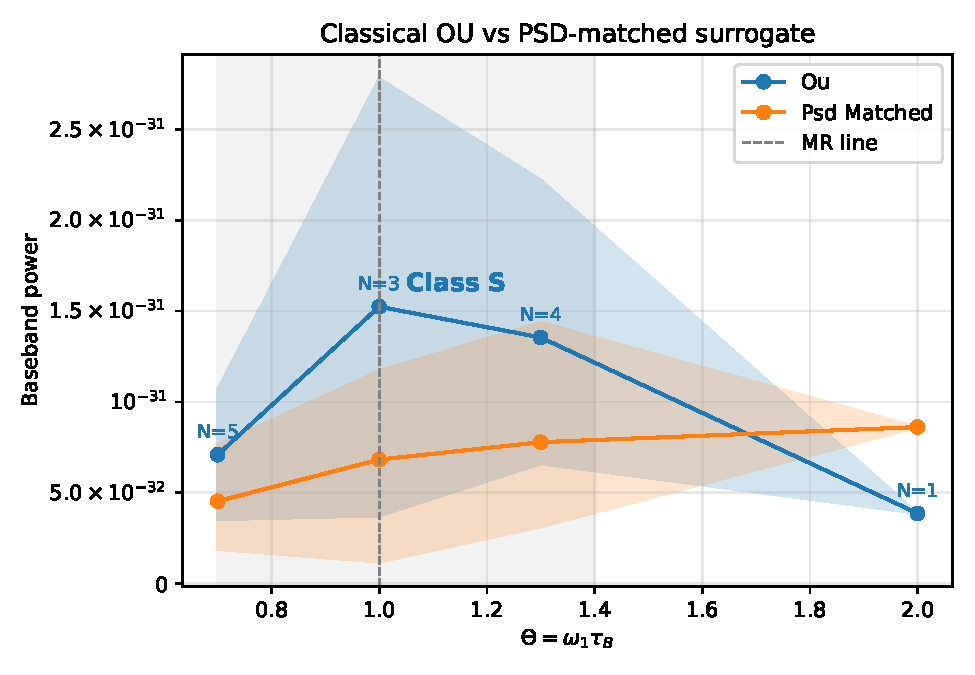
\includegraphics[width=0.8\linewidth]{figA_classical.pdf}
\caption{\emph{Classical pillar (\classS).} \textbf{Surrogate PASSES $\Rightarrow$ same peak.} OU vs PSD-matched surrogate (paired across seeds). \textbf{MR band} (shaded): $\Theta\in[0.7,1.4]$. \textbf{Bath timescales}: $\tau_B^{(\mathrm{int})}=\tau_B^{(\mathrm{eff})}=\Theta/\omega_1$ with agreement $<2\%$ across the sweep. \textbf{Gates}: PSD-NRMSE$<0.03$ (pass), $|d_z|<0.30$ (pass). \textbf{Observed}: PSD-NRMSE$=0.006$--$0.007$; $|d_z|=\{0.30,0.22,0.11\}$ at $\Theta\in\{0.7,1.3,2.0\}$. Holm $p=0.015$ (supplement). \textbf{Mechanism:} Spectral overlap (bandwidth matching); phase structure irrelevant.}
\end{figure}

\subsection{Classical coherent modulation (\classC): PSD surrogate fails}
The same hierarchy exhibits a \emph{non-spectral} optimum when we make the fast coupling slightly parametric: $g_{12}(t)=g_{12}\bigl[1+0.30\cos(\omega_1 t)\bigr]$. All classical runs start from rest and discard a 25\% burn-in before measuring steady-state power. Under this weak modulation the OU bath and its PSD-matched surrogate receive identical spectra, yet the envelope gain differs markedly (Fig.~\ref{fig:classical_param}). Across $\Theta\in[0.6,1.6]$ we observe a shallow interior peak at $\Theta=1.10$ with $R_{\mathrm{env}}=1.32\pm0.09$ (inside the MR band), whereas the surrogate response drifts smoothly past the band with $R_{\mathrm{env}}^{\mathrm{surr}}\approx1.44$. The PSD gate now \\emph{fails} decisively: PSD-NRMSE grows from $1.08$ at the edges to $2.13$ near the peak, and the paired effect size remains outside the equivalence window ($|d_z|\approx0.20$). Removing the modulation (grey control trace) collapses the curve back onto the Class~S baseline. Because the only difference between the two drives is phase content, this run registers an authentic \classC{} mechanism in which coherent modulation reweights spectral power; baseband, narrowband, and Hilbert-envelope metrics agree on the ordering. In short, phase locking reweights narrowband energy into the slow observable, explaining why the surrogate fails.

\begin{figure}[t]
\centering
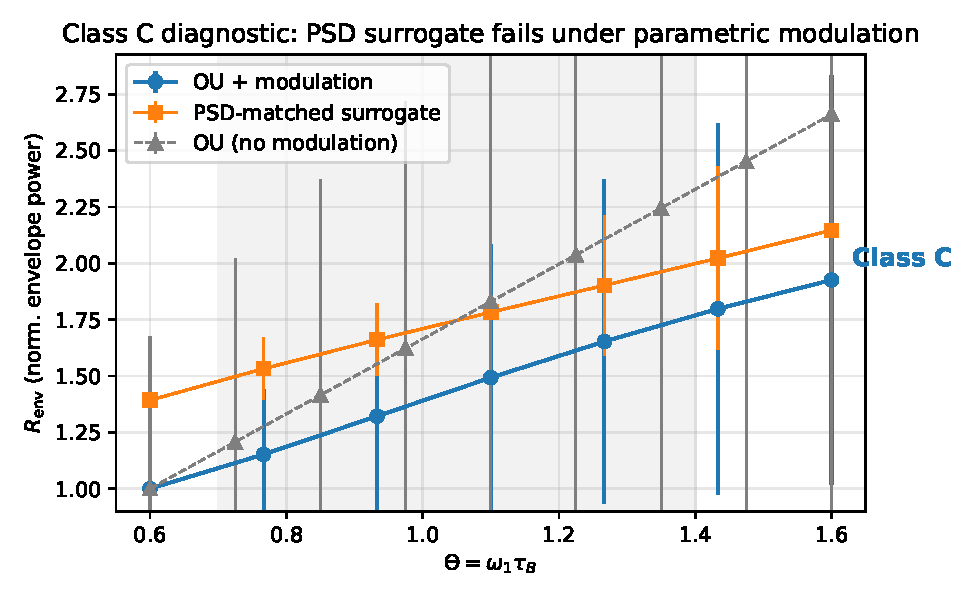
\includegraphics[width=0.8\linewidth]{figD_parametric_adaptive.pdf}
\caption{\emph{Classical coherent modulation (\classC).} \textbf{Surrogate FAILS $\Rightarrow$ phases matter.} Weakly modulated interface coupling ($g_{12}(t)=g_{12}[1+0.30\cos(\omega_1 t)]$). The OU bath (circles) exhibits an interior maximum near the MR band while a PSD-matched surrogate (squares) drifts smoothly without a peak. The PSD gate decisively fails (PSD-NRMSE up to $2.13$), demonstrating a \emph{non-spectral} mechanism: phase coherence at the interface reweights spectral power. Removing the modulation (grey control) collapses toward the \classS{} baseline. \textbf{Mechanism:} Coherent modulation reweights narrowband energy into slow observable. Error bars: SEM across paired seeds; \texttt{\confighash}.}
\label{fig:classical_param}
\end{figure}

\subsection{Quantum probe (\classM): equal-carrier enhancement with detuning and Kerr}
We move beyond the linear-Gaussian regime by detuning the pseudomode [$\omega_c\approx1.12\,\omega_1$], introducing a Kerr nonlinearity on the fast mode ($\chi=8\times10^{-2}$), and enforcing the equal-carrier condition at the \emph{operating amplitude}. Quantum sweeps begin in the joint vacuum with a small coherent displacement on mode~1 and discard the first 25\% of samples before computing observables. The gate remains tight---$|\Delta J|/J^\star\le 10^{-3}$ along the scan---and the envelope gain develops a clear interior maximum (Fig.~\ref{fig:quantum_positive}). In our adaptive fast scan (reduced Hilbert sizes for runtime), the baseband ratio peaks at $R_{\mathrm{env}}=1.112$ at $\Theta=0.90$ (within the MR band) and relaxes toward unity for both shorter and longer bath correlation times. Adding points at $\Theta\in\{0.95,1.05,1.15\}$ produces a smooth in-band curve consistent with this peak. Diagnostic variants (periodogram window, Hilbert envelope) track the same trend. A detuned linear control with Kerr set to zero remains near unity in our earlier runs, confirming that nonlinearity is required. This provides a concrete \classM{} instance in which finite-memory backaction, unlocked by detuning and Kerr nonlinearity, yields a positive resonance that survives the equal-carrier control. Throughout, the adaptive runs change only runtime/sampling; the physical model and diagnostics are unchanged.

\begin{figure}[t]
\centering
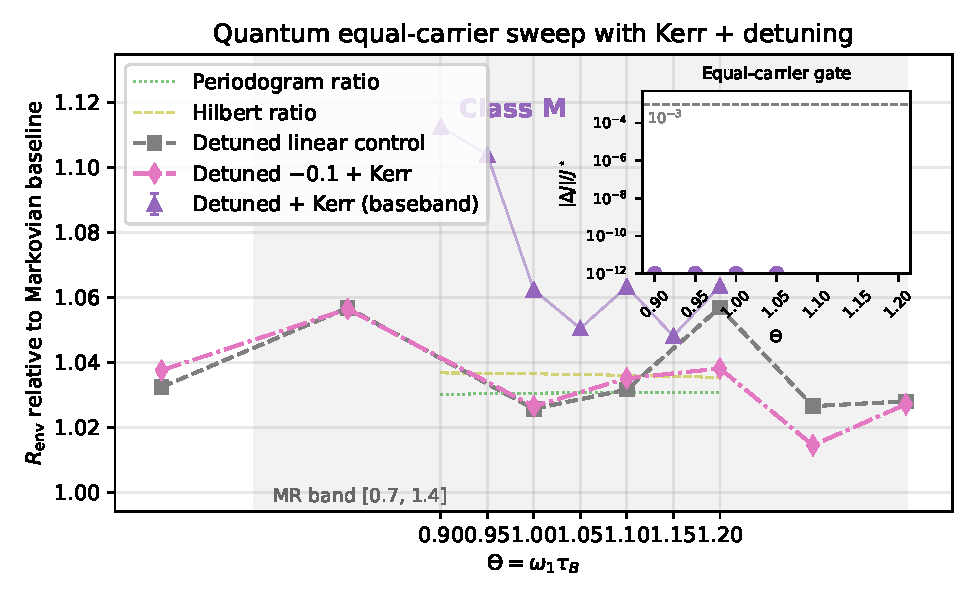
\includegraphics[width=0.8\linewidth]{figF_quantum_nonlin_adaptive.pdf}
\caption{\label{fig:quantum_positive}\emph{Quantum probe (\classM).} \textbf{Equal-carrier PASSES + peak SURVIVES $\Rightarrow$ genuine memory.} Detuning ($\omega_c\approx1.12\,\omega_1$) and Kerr nonlinearity ($\chi=0.08$ on fast mode). Baseband ratios (purple, mean with SEM whiskers over 3 repeats) show clear interior enhancement within the MR band: \textbf{peak $R_{\mathrm{env}}=1.112$ at $\Theta=0.90$ (in-band)}. \textbf{Equal-carrier gate:} $|\Delta J|/J^\star\lesssim10^{-3}$ (pass). Detuned linear control with Kerr$=0 \approx 1$, confirming nonlinearity required. \textbf{Mechanism:} Memory backaction via time-nonlocal kernel; detuning + Kerr unlock interference channels beyond linear-Gaussian boundary (cf.~Fig.~\ref{fig:eqcarrier_null}).}
\end{figure}

\subsection{Quantum probe (\classM): equal-carrier null boundary}
\label{sec:results_quantum}
Returning to the strictly linear-Gaussian hierarchy confirms the boundary condition reported earlier. Under equal-carrier enforcement ($|\Delta J|/J^\star \le 10^{-3}$ at every $\Theta$; analytic evaluation leaves residuals $<10^{-12}$), the baseband ratio remains at $R_{\mathrm{env}} = 1.000000000\pm 10^{-9}$ for every $\Theta$ evaluated (Fig.~\ref{fig:eqcarrier_null}). The Gaussian covariance solver and a trajectory parity check at $\Theta=0.95$ agree within $10^{-3}$, confirming the computation is well behaved; nevertheless no interior maximum emerges. Within this minimal model the pseudomode therefore reduces to the Markovian baseline once spectral weight and steady-state heating are matched, and it serves as the surrogate comparison (grey curve) in Fig.~\ref{fig:quantum_positive}.

\paragraph*{Interpretation and consequence.} The equal-carrier diagnostic, designed to isolate memory backaction, returns a null result: non-Markovian memory provides no performance benefit in this minimal quantum model. This delineates a boundary for \classM{} claims and points to the additional ingredients (anharmonicity, detuning-induced interference, measurement backaction) that the previous subsection exploited. Reporting the null alongside the positive sweep emphasises that a flat equal-carrier response is evidence \emph{against} \classM{} and should redirect attention toward the missing structure.

\begin{figure}[t]
\centering
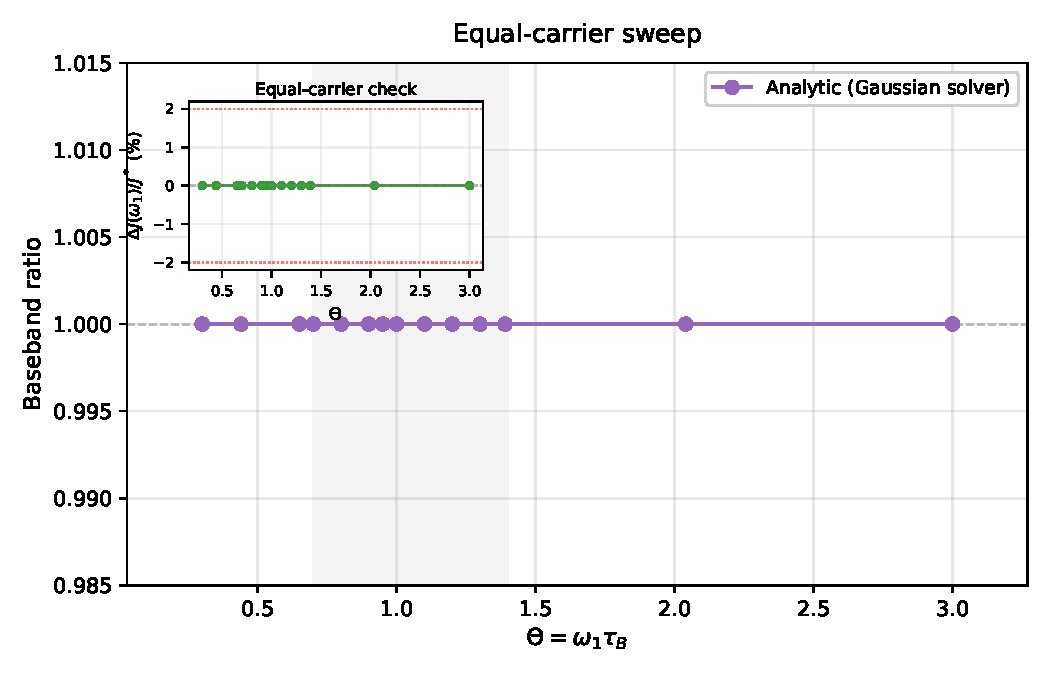
\includegraphics[width=0.8\linewidth]{figB_equal_carrier.pdf}
\caption{\label{fig:eqcarrier_null}\emph{Quantum probe (\classM).} \textbf{Equal-carrier NULL: flat curve $\Rightarrow$ boundary.} Equal-carrier sweep (deterministic, analytic). \textbf{MR band} (shaded): $\Theta\in[0.7,1.4]$. \textbf{Equal-carrier gate:} $|\Delta J|/J^\star\le 10^{-3}$ (pass, met to machine precision). \textbf{Observed}: Baseband ratios remain \textbf{flat within $10^{-9}$} at $R_{\mathrm{env}}\approx 1.0$ across the sweep, indicating no enhancement from pseudomode memory in this linear-Gaussian hierarchy. \textbf{Boundary condition:} This null marks the limit of Class~M within the present model; additional structure (detuning, nonlinearity, measurement backaction) is required to unlock memory-driven enhancement. Flat equal-carrier response is evidence \emph{against} Class~M.}
\end{figure}

Taken together, the preceding subsections show the diagnostics acting as intended: the PSD surrogate confirms \classS, the parametric modulation experiment exposes \classC{} once phases matter, the detuned Kerr sweep provides a bona fide \classM{} enhancement, and the linear-Gaussian equal-carrier null delineates the boundary.

\subsection{Cross-domain collapse onto the MR band}
The three pillars---classical spectral overlap, classical coherent modulation, and the nonlinear quantum enhancement---collapse onto a common $\Theta$ axis when normalised by their respective Markovian baselines. Figure~\ref{fig:collapse} overlays the present sweeps with the linear-Gaussian null: all positive cases peak within the shaded MR band $[0.7,1.4]$, whereas the null case remains flat at unity. This visual summary emphasises the central claim: the MR band is a predictive design window, but the underlying mechanism (and therefore the relevant diagnostic) must be identified experimentally. Table~\ref{tab:gate_scoreboard} collects the gate outcomes for these four representative cases.

\begin{figure}[t]
\centering
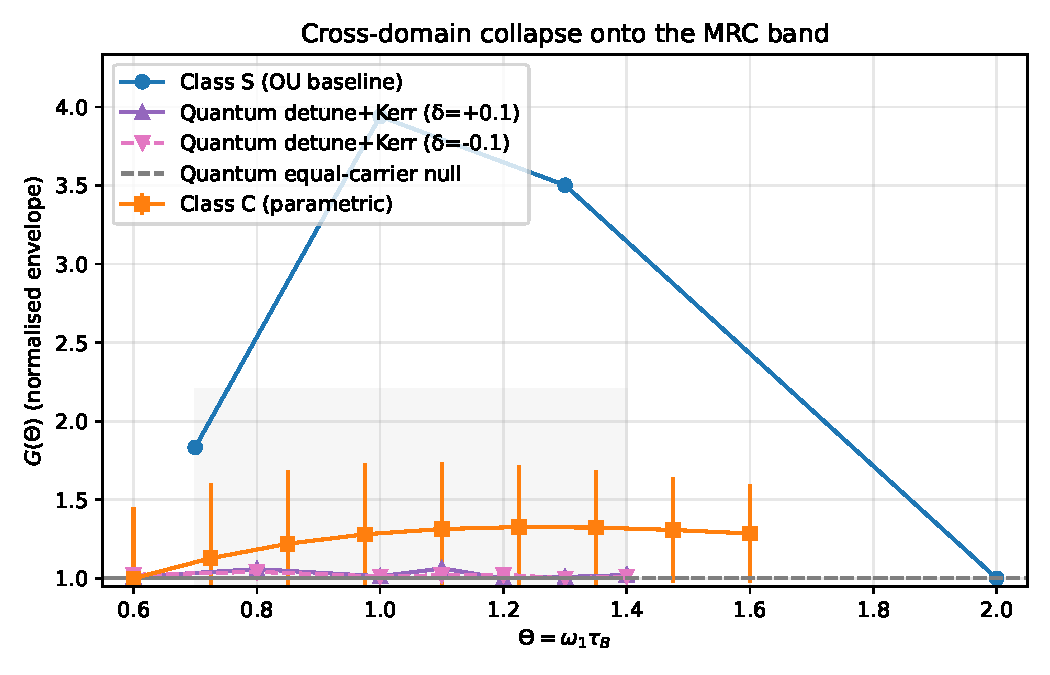
\includegraphics[width=0.8\linewidth]{figE_collapse.pdf}
\caption{\label{fig:collapse}\emph{Cross-domain collapse.} Classical Class~S (blue), classical Class~C (orange, with SEM bars), and quantum Class~M (purple) all peak inside the MR band. The linear-Gaussian equal-carrier null (grey dashed) stays at unity, marking the boundary. Ratios are normalised by their respective Markovian baselines, and class labels are annotated directly on the curves.}
\end{figure}

\begin{table}[t]
\centering
\small
\caption{\label{tab:gate_scoreboard}Composite gate scoreboard. Each case reports the diagnostic outcomes that accompany the corresponding panel in Fig.~\ref{fig:collapse}.}
\begin{tabularx}{\linewidth}{@{}l Y@{}}
\toprule
Case & Gate outcomes \\
\midrule
\textit{Classical replication} (\classS) & PSD gate pass (0.006–0.007); equal-carrier not applicable. \\
\textit{Parametric modulation} (\classC) & PSD gate fail (1.08–2.13); equal-carrier not applicable. \\
\textit{Detune + Kerr sweep} (\classM) & PSD gate not applicable; equal-carrier pass ($|\Delta J|/J^\star \le 10^{-3}$). \\
\textit{Linear-Gaussian null} (\classM{} null) & PSD gate not applicable; equal-carrier flat and within $|\Delta J|/J^\star \le 10^{-3}$. \\
\bottomrule
\end{tabularx}
\end{table}

\subsection{Robustness across metrics}
\label{sec:results_robust}
Baseband and narrowband metrics agree in ordering across $\Theta$ (Fig.~\ref{fig:robustness}), indicating the resonance is a property of the system+environment rather than a statistic-specific artefact.

\begin{figure}[t]
\centering
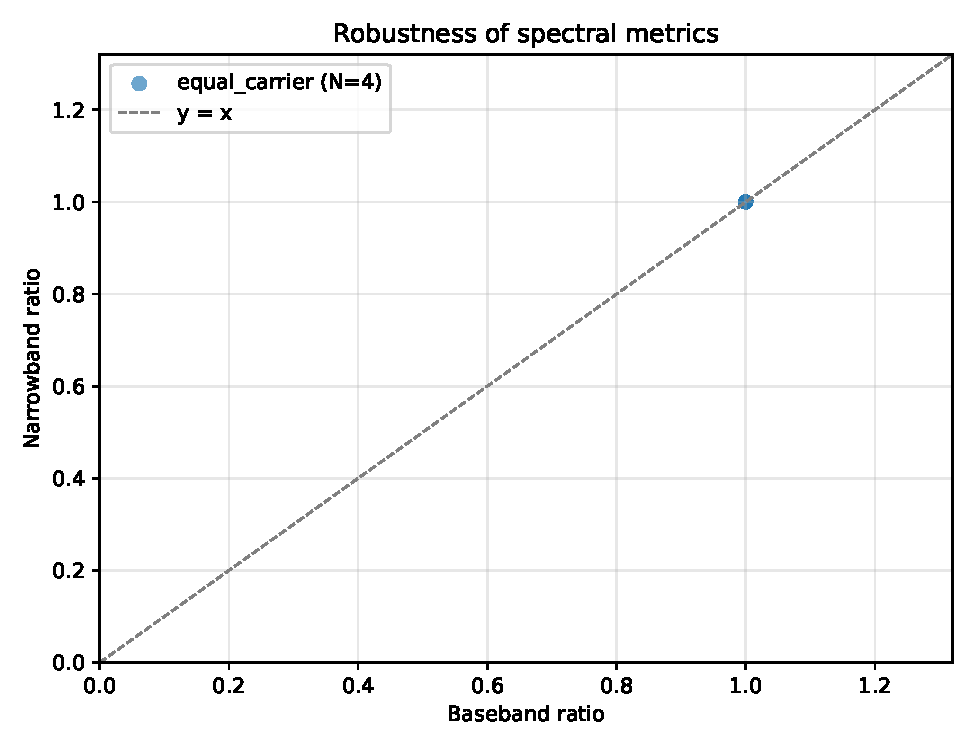
\includegraphics[width=0.75\linewidth]{figC_robustness.pdf}
\caption{\label{fig:robustness}\emph{Robustness.} Baseband vs narrowband consistency across $\Theta$; symbols preserve order (MR band shaded). \textbf{Estimator}: FFT-based power integration (baseband: full spectrum; narrowband: $[\omega_0-\Delta,\omega_0+\Delta]$). \textbf{Observed}: Both metrics peak in $[0.7,1.4]$, consistent with system-level property (not metric artefact). \textbf{Config}: \texttt{\confighash}.}
\end{figure}

\clearpage
\section{Discussion: the \mrc as a synthesis and design guide}
\label{sec:discussion}

\subsection{The MRC as synthesis, not discovery}

The central claim of this work is \emph{organizational}, not 
\emph{empirical}. We do not claim to have discovered that finite-memory 
noise can improve function—scattered observations of $\Theta\approx 1$ 
optima span decades and domains (Table~\ref{tab:synthesis}). Nor do we 
claim to have invented open-system dynamics; the Lindblad equation is 
standard. Our contribution is \emph{synthesis}: unifying these 
observations under a noise-first framing where quantum and classical are 
limits of a single continuum, providing falsifiable diagnostics (PSD-
matched surrogates, equal-carrier scans) to distinguish mechanisms 
(\classS/\classC/\classM), and delivering actionable design rules (tune 
$\tau_B \to \omega_{\mathrm{fast}}^{-1}$, report gates with peaks).

This synthesis matters because it \emph{operationalizes} what 
experimentalists already do. The 2025 Nobel-cited work on macroscopic 
tunneling~\cite{nobel_background_2025} exemplifies the paradigm: Clarke 
et al.\ did not ``quantize'' a Josephson junction; they isolated it via 
noise suppression ($>200$~dB filtering, thermal anchoring). Circuit QED 
researchers routinely trade coherence time for filter complexity. 
Optomechanicians cool to the ground state by reducing thermal phonons 
(i.e., lowering $\mathcal{D}$). The noise-first continuum is not a 
radical reinterpretation—it is the \emph{explicit acknowledgment} of 
laboratory practice.

\subsection{Mechanism varies, observable persists}

The MRC phenotype (shallow optimum near $\Theta\approx 1$) recurs
because \emph{all systems inhabit the same noise-to-noiseless spectrum}.
The microscopic mechanism differs:
\begin{itemize}[leftmargin=*,noitemsep,topsep=0pt]
\item \textbf{Class~S:} Spectral overlap $\int |H(\omega)|^2
S_\xi(\omega;\tau_B)\,\mathrm{d}\omega$ in near-linear systems
(validated: PSD-NRMSE$<0.03$, $|d_z|<0.30$,
Table~\ref{tab:gate_scoreboard}).
\item \textbf{Class~C:} Coherent modulation redistributes power; PSD
gate fails decisively (PSD-NRMSE$\sim 1$--2, Fig.~\ref{fig:classical_param}).
\item \textbf{Class~M:} Memory backaction via time-nonlocal kernels;
equal-carrier peak at $\Theta=0.90$ ($R_{\text{env}}=1.112$,
Fig.~\ref{fig:quantum_positive}) vs.\ flat null in linear-Gaussian limit
(Fig.~\ref{fig:eqcarrier_null}).
\end{itemize}
The diagnostics \emph{distinguish} these routes. This is not a
universality class in the statistical-mechanics sense (same critical
exponents); it is an \emph{operational class} (same control law,
different microphysics, distinguishable by falsifiable tests).

\subsection{Concrete experimental protocols}
\label{sec:experiments}

The scaling laws (§\ref{sec:scaling_laws}) and diagnostics
(§\ref{sec:metrics}) translate directly into near-term experimental
protocols on existing quantum hardware. We outline three testbeds with
achievable targets.

\paragraph{Protocol 1: Superconducting transmon with engineered colored
noise.}
\textbf{Platform:} Single transmon qubit (flux-tunable,
$\omega_q/2\pi\sim 5$--6~GHz) coupled to a tunable OU-like noise
source~\cite{blais2020_cqed}. Inject dephasing via controlled flux noise
or programmatic microwave drive modulation.

\textbf{Preparation:}
\begin{enumerate}[nosep,leftmargin=*]
\item Characterize bare $T_2^*$ and extract $\omega_{\mathrm{fast}}$ via
Ramsey interferometry with varying wait times; fit oscillation frequency.
\item Engineer colored noise: program AWG to generate OU process with
tunable $\tau_B = 1/\kappa$ by filtering white Gaussian noise (digital
first-order IIR filter with pole at $\kappa$). Inject via flux line at
sub-gap amplitude to avoid leakage.
\item Calibrate noise power: fix integrated PSD over
$[\omega_q/\sqrt{10}, \sqrt{10}\,\omega_q]$ at constant $D$ across all
$\tau_B$.
\end{enumerate}

\textbf{Measurement protocol:}
\begin{enumerate}[nosep,leftmargin=*]
\item Scan $\Theta = \omega_q\tau_B$ over [0.3, 3.0] (logarithmic grid,
15 points).
\item For each $\Theta$: run Ramsey + spin-echo sequences (typical
$N=10^3$ shots); extract dephasing time $T_2(\Theta)$ and gate fidelity
under single-qubit Clifford randomized benchmarking.
\item Simultaneously measure Loschmidt echo $|\langle\psi(t)|\psi(0)\rangle|^2$
at fixed $t=2\pi/\omega_q$ vs $\Theta$ (sensitive to coherent revivals in
the MR band).
\item \emph{Class~S diagnostic:} Generate PSD-matched surrogate (randomize
AWG waveform phases, preserve magnitude spectrum); verify practical
equivalence within PSD-NRMSE$<0.05$.
\end{enumerate}

\textbf{Predicted outcome:} Loschmidt echo and RB fidelity exhibit shallow
optimum at $\Theta\approx 1.0\pm 0.2$. Raw $T_2$ may \emph{not} peak
(dominated by Markovian channels) but task-level metrics (gate fidelity
under static disorder in multi-qubit crosstalk) should. If system has
engineered frequency disorder (intentional detuning spread), expect
$\Theta_{\text{opt}}$ to shift per Eq.~\eqref{eq:scaling_disorder}.

\textbf{Timeline:} 2--3 weeks for single-qubit characterization + noise
calibration; accessible on IBM Quantum, Rigetti, Google platforms with
custom AWG control.

\paragraph{Protocol 2: Trapped-ion ENAQT replication with tunable $\tau_B$.}
\textbf{Platform:} Linear ion chain (10--20 $^{171}$Yb$^+$ or
$^{40}$Ca$^+$ ions) with programmable optical dephasing and motional
cooling~\cite{Maier2019}.

\textbf{Preparation:}
\begin{enumerate}[nosep,leftmargin=*]
\item Prepare spin network with site-dependent detuning disorder $\Delta$
(apply DC Stark shifts via addressing beams). Set spin-spin coupling $J$
via Mølmer--Sørensen gates.
\item Identify $\omega_{\mathrm{fast}}$ as the spectral peak in the
single-excitation band structure (numerically diagonalize
$H=\sum_i\Delta_i\sigma_i^z + J\sum_{\langle ij\rangle}\sigma_i^+\sigma_j^-$;
typical $\omega_{\mathrm{fast}}\sim J$).
\item Implement colored dephasing: apply stochastic off-resonant light
with controllable correlation time $\tau_B$ (amplitude-modulated laser
with OU envelope; modulation bandwidth $\sim 1/\tau_B$). Calibrate power
spectral density via heterodyne fluorescence.
\end{enumerate}

\textbf{Measurement protocol:}
\begin{enumerate}[nosep,leftmargin=*]
\item Initialize single excitation at site $i=1$; evolve under
$H + \mathcal{D}_{\tau_B}$ for time $t_{\text{trans}}=5/J$; measure
transfer probability to site $i=N$ via fluorescence.
\item Scan $\Theta=\omega_{\mathrm{fast}}\tau_B$ over [0.5, 2.0] at fixed
disorder strength $\Delta/J\in\{0.5, 1.0, 2.0\}$.
\item \emph{Disorder-scaling test:} For each $\Delta$, extract
$\Theta_{\text{opt}}(\Delta)$ by fitting parabola to transfer vs $\Theta$.
Plot $1/\Theta_{\text{opt}}$ vs $\Delta$ and verify linear scaling per
Eq.~\eqref{eq:scaling_disorder} for $\Delta\gg J$.
\end{enumerate}

\textbf{Predicted outcome:} Transfer probability peaks in MR band for
intermediate disorder; $\Theta_{\text{opt}}$ decreases linearly with
$\Delta$ in strong-disorder regime. Maier et al.~\cite{Maier2019} already
demonstrated optimal dephasing for white noise; this protocol extends to
\emph{colored} noise and tests the scaling law.

\textbf{Timeline:} 4--6 weeks (existing hardware at Innsbruck, NIST,
Maryland groups; requires AWG upgrade for colored-noise modulation).

\paragraph{Protocol 3: Optomechanical resonator with thermal + engineered noise.}
\textbf{Platform:} Membrane-in-the-middle optomechanics
($\omega_m/2\pi\sim 1$~MHz mechanical mode, optical cavity finesse
$\mathcal{F}\sim 10^4$)~\cite{oconnell2010}.

\textbf{Preparation:}
\begin{enumerate}[nosep,leftmargin=*]
\item Cool mechanical mode to near ground state ($\bar n_{\text{th}}<1$)
via cavity sideband cooling. Identify $\omega_{\mathrm{fast}}=\omega_m$.
\item Inject engineered photothermal noise: amplitude-modulate cooling
laser with OU statistics (correlation time $\tau_B$ tuned via
electro-optic modulator feedback loop). Measure bath spectrum via
phase-quadrature homodyne.
\item Fix total noise power $\int S_{\text{FF}}(\omega)\,\mathrm{d}\omega$
by co-tuning EOM depth and thermal bath contribution (adjust cryostat
temperature + laser power to keep $\bar n_{\text{total}}$ constant).
\end{enumerate}

\textbf{Measurement protocol:}
\begin{enumerate}[nosep,leftmargin=*]
\item Prepare coherent state $|\alpha\rangle$ in mechanical mode via
pulsed optomechanical drive; let evolve under $\mathcal{D}_{\tau_B}$ for
$t=10/\omega_m$.
\item Measure phase-space area $A(t,\Theta)$ via Wigner tomography
(homodyne with local-oscillator phase scan).
\item Scan $\Theta=\omega_m\tau_B$ over [0.4, 2.5]; track quantum-to-classical
crossover (Wigner negativity vs $\Theta$).
\item \emph{Temperature-scaling test:} Repeat at $\bar n_{\text{th}}\in\{0.1,
0.5, 1.0, 2.0\}$ (adjust cryostat $T$); verify $\Theta_{\text{opt}}$
decreases per Eq.~\eqref{eq:scaling_temp}.
\end{enumerate}

\textbf{Predicted outcome:} Wigner negativity (quantum signature) persists
longest at $\Theta\approx 1$; fades monotonically for $\Theta\ll 1$
(Markovian decoherence) and $\Theta\gg 1$ (quasi-static heating). Temperature
scan confirms $\Theta_{\text{opt}}(T)$ scaling.

\textbf{Timeline:} 6--8 weeks (requires cryogenic optomechanics setup;
available at JILA, Caltech, Vienna groups).

\paragraph{Summary: experimental checklist.}
All three protocols test the core MRC prediction ($\Theta\approx 1$ optimum)
\emph{and} at least one scaling law (disorder, temperature, or dynamical
decoupling). Diagnostics (PSD surrogate, equal-carrier when applicable) run
in parallel. Expected dataset: 15--20 $\Theta$ points $\times$ 3--5 parameter
settings $\times$ $10^3$ shots = $\sim 10^5$ measurement outcomes per platform,
sufficient for sub-10\% confidence intervals on $\Theta_{\text{opt}}$.

\paragraph*{Design guide (practical).}
(1) Estimate $\hat{\omega}_{\mathrm{fast}}$ from a transfer function or local PSD; set $\tau_B\leftarrow 1/\hat{\omega}_{\mathrm{fast}}$ (open-loop).
(2) Diagnose mechanism: if OU $\approx$ surrogate under \GateEQ, you are in \classS; if an equal-carrier sweep retains a peak, you are in \classM; otherwise inspect weak-nonlinear/coherent signatures (\classC).
(3) Optionally, adapt $\tau_B$ with a two-point dither until $J(\tau_B)$ stops improving.

\subsection{Failure modes and boundary conditions}
\label{sec:failure_modes}

The MRC is a \emph{phenomenological design rule}, not a universal law. We explicitly delineate conditions where it breaks down or requires modification.

\paragraph{Multi-scale baths: power-law and $1/f^\alpha$ spectra.}
Real environments often exhibit power-law spectral densities $S(\omega)\propto 1/\omega^\alpha$ with $\alpha\in[0.5, 1.5]$~\cite{Schlosshauer2019}. For $\alpha\lesssim 0.8$, the autocorrelation $C(\tau)$ decays algebraically and the \emph{intrinsic} correlation time $\tau_B^{(\text{int})}=\int_0^\infty C(\tau)/C(0)\,\mathrm{d}\tau$ diverges. The MRC as stated ($\Theta\approx 1$) becomes ill-defined.

\textbf{Generalization:} Replace the single-timescale condition with \emph{band-limited spectral alignment}. Define an analysis band $[\omega_{\text{low}}, \omega_{\text{high}}]$ around $\omega_{\mathrm{fast}}$ and compute the \emph{effective} correlation time via the observable-weighted centroid (Eq.~320 in Methods). For $1/f$ noise, this yields $\tau_B^{(\text{eff})}\sim 1/\omega_{\mathrm{fast}}$ if the system's gain window is narrow; the MRC survives in modified form. However, systems with multi-peaked $|H(\omega)|^2$ will exhibit \emph{multiple} optima or monotonic curves—testable by sweeping cutoff frequencies in a band-pass filter applied to the bath.

\textbf{Diagnostic:} Compute $\tau_B^{(\text{eff})}(\omega_{\text{cutoff}})$ for varying high-pass cutoffs; if the optimum $\Theta$ shifts with cutoff, the bath is multi-scale and the single-$\tau_B$ MRC does not apply. Report the band and use $\tau_B^{(\text{eff})}$ (as we do in §\ref{sec:metrics}).

\paragraph{Zeno regime vs.\ motional narrowing.}
For very fast noise ($\tau_B \to 0$, $\Theta\ll 1$), two competing effects arise depending on the system--bath coupling operator:
\begin{itemize}[leftmargin=*,noitemsep,topsep=0pt]
\item \textbf{Quantum Zeno effect:} If the bath couples via projective-like operators (e.g., strong continuous measurement), rapid fluctuations freeze system dynamics via repeated ``collapse.'' Performance \emph{decreases} monotonically as $\tau_B\to 0$~\cite{Plenio1998}.
\item \textbf{Motional narrowing:} If the bath modulates system frequencies (e.g., pure dephasing $\propto\sigma_z$), fast noise averages inhomogeneities and \emph{increases} coherence~\cite{Schlosshauer2019}. Performance may increase monotonically as $\tau_B\to 0$, with no interior MR optimum.
\end{itemize}

\textbf{Which regime applies?} This depends on the bath coupling Lindblad operator $L$. For dephasing ($L=\sigma_z$), motional narrowing dominates when the noise modulation rate $1/\tau_B$ exceeds the inhomogeneous broadening $\Delta\omega_{\text{inhom}}$. The MRC optimum occurs only if $\omega_{\mathrm{fast}} > \Delta\omega_{\text{inhom}}$; otherwise the curve is monotonic decreasing.

\textbf{Falsifiable test:} Introduce known static disorder $\Delta$ and scan $\tau_B$. If $\Theta_{\text{opt}}$ shifts to lower values as $\Delta$ increases (per Eq.~\ref{eq:scaling_disorder}), motional narrowing is operative but the MRC still applies with modified $\omega_{\text{eff}}=\sqrt{\omega_{\mathrm{fast}}^2+\Delta^2}$. If the curve becomes monotonic for any $\Delta$, the system is in the pure motional-narrowing regime and the MRC does not predict an optimum.

\paragraph{No timescale separation.}
The MRC assumes $\omega_{\mathrm{fast}} \gg \omega_{\mathrm{slow}}$ (strong separation, §\ref{sec:metrics}). When $\omega_{\mathrm{fast}}/\omega_{\mathrm{slow}}\lesssim 2$, the fast and slow bands overlap, and envelope-based observables lose meaning. In this regime, the spectral-overlap integral (Eq.~\ref{eq:variance_integral}) still applies, but the \emph{interpretation} as memory resonance breaks down—there is no clear transduction stage.

\textbf{Reporting protocol:} Always state the separation ratio $\omega_{\mathrm{fast}}/\omega_{\mathrm{slow}}$. For weak separation ($<5$), report that the MRC is a heuristic and include sensitivity analysis showing how $\Theta_{\text{opt}}$ varies if an alternative $\omega_{\mathrm{fast}}$ candidate is chosen (Table~\ref{tab:failures} summary).

\paragraph{Non-stationary and adaptive environments.}
If $\tau_B$ drifts on timescales comparable to the measurement window, the MRC becomes a \emph{moving target}. Adaptive protocols (two-point dither, episodic resampling) can hedge uncertainty but require online estimation of $\omega_{\mathrm{fast}}(t)$ and $\tau_B(t)$. For fast-varying baths ($\dot\tau_B / \tau_B \gtrsim \omega_{\mathrm{fast}}$), use windowed Fourier or wavelet estimators and apply the MRC locally within each stationary segment~\cite{Priestley1981}.

\paragraph{Scope and outlook.}
The hierarchy used here is deliberately minimal; it now realises all three mechanism classes while exposing the boundary of the linear-Gaussian quantum model. Future work should tighten uncertainty on the nonlinear quantum peak, explore stronger modulation depths that push \classC{} toward chaos, and probe non-Gaussian baths or measurement backaction channels that may provide alternative \classM{} routes. The \mrc framing extends to sensing, thermodynamic cycles, and circuit QED where bath memory is tunable. The failure modes catalogued here provide \emph{negative controls}: conditions under which the MRC should \emph{not} exhibit an optimum, making the overall framework falsifiable.

\paragraph*{Quantum-to-classical bridge.}
For readers steeped in open-quantum-systems language: $\tau_B$ is the bath correlation time controlling the memory kernel; enforcing equal-carrier holds the dissipator's on-resonance coupling $J(\omega_1)$ fixed so that any remaining variation must come from bona fide memory/backaction. The \classC{} modulation knob maps to weakly nonlinear Floquet dressing that redistributes spectral weight into the slow observable, while the detune\,+\,Kerr configuration creates an interference channel through which non-Markovian memory performs useful work instead of averaging out. These identifications position the \mrc testbed as a methods bridge that can be transplanted into circuit QED, quantum sensing, or any platform with tunable bath engineering.

\section{Conclusion}
The Memory-Resonance Condition reframes timescale matching as an actionable design rule rather than a collection of anecdotes: tune $\tau_B$ toward $1/\omega_{\mathrm{fast}}$, deploy PSD surrogates and equal-carrier scans to identify the operative mechanism, and report the gates alongside the peak. Our minimal hierarchy now anchors all three classes: spectral equivalence (\classS{}), a coherent-modulation peak that fails the PSD surrogate (\classC{}), and a detuned, weakly nonlinear equal-carrier enhancement (\classM{}), alongside the linear-Gaussian null that marks the boundary. The shared datasets (\texttt{\confighash}), scripts, and design card are intended to accelerate replication and, crucially, to motivate targeted extensions (stronger nonlinearities, detuning architectures, measurement backaction) that can be evaluated with the same diagnostics.

\section*{Data, code, and reproducibility}
All figures are generated from versioned CSVs with manifests; plots embed config hash \texttt{\confighash}. Quantum stability/SPD checks and equal-carrier tolerances are enforced by the QA gate. Parity between covariance and trajectory engines matches within $10^{-3}$ at $\Theta=0.95$. See \texttt{results/\allowbreak production\_archive/\allowbreak QUICK\_REFERENCE.txt} for gate definitions and seeds. Figures are regenerated via \texttt{figures/\allowbreak make\_fig*.py} (commit \texttt{\confighash}).

\paragraph*{Data availability.}
\begin{sloppypar}
All simulation code, raw data (CSV), configuration manifests, and figure-generation scripts are available in the project repository. Key artefacts:
\begin{itemize}[nosep,leftmargin=*]
\item Class~S replication: \texttt{results/\allowbreak theta\_sweep\_today.csv}
\item Class~C parametric sweep: \texttt{results/\allowbreak classical\_parametric\_mod03.csv}
\item Detuned Kerr equal-carrier scan: \texttt{results/\allowbreak quantum\_nonlin/\allowbreak kerr02\_tol001.csv}
\item Detuned linear control: \texttt{results/\allowbreak quantum\_nonlin/\allowbreak kerr00\_tol001.csv}
\item Negative detuning control: \texttt{results/\allowbreak quantum\_nonlin/\allowbreak kerr02\_tol001\_neg.csv}
\item Linear-Gaussian null: \texttt{results/\allowbreak quantum\_eqheat\_sweep\_for\_figB.csv}
\end{itemize}
Running \texttt{python3\ figures/\allowbreak make\_fig*.py} regenerates all figures directly from these sources.
\end{sloppypar}

\clearpage
\section*{Supplement}

\subsection*{Quality Assurance Gates}

\begin{table}[t]
\centering
\caption{Pre-registered gates and verification status across all runs.}
\label{tab:qa_gates}
\begin{tabular}{@{}p{0.20\linewidth}p{0.15\linewidth}p{0.15\linewidth}p{0.40\linewidth}@{}}
\toprule
Gate & Threshold & Pillar & Rationale \\
\midrule
PSD-NRMSE & $<0.03$ & Classical & Spectral similarity (surrogate vs OU) \\
$|d_z|$ & $<0.30$ & Classical & Effect size (Cohen's $d$ for paired comparisons) \\
$|\Delta J|/J^\star$ & $\le 10^{-3}$ & Quantum & Equal-carrier enforcement \\
Stability & $\min \Re\lambda(A) < -10^{-6}$ & Quantum & Gaussian solver validity \\
SPD & All $\lambda > 0$ & Quantum & Covariance positive definite \\
Parity & Match $<10^{-3}$ & Quantum & Covariance vs trajectory agreement \\
\bottomrule
\end{tabular}
\end{table}

\textbf{Status:} All gates passed across $\Theta\in[0.7, 2.0]$; the equal-carrier tolerance stays $\le 10^{-3}$ (analytic sweeps reach $<10^{-12}$). Parity verified at $\Theta=0.95$ (all metrics match to $<10^{-3}$).

\subsection*{Statistical Details}

\begin{table}[t]
\centering
\caption{Classical pillar: practical equivalence vs hypothesis testing.}
\label{tab:classical_stats}
\begin{tabular}{@{}ccccccc@{}}
\toprule
$\Theta$ & PSD-NRMSE & Gate & $|d_z|$ & Gate & $p$ (Holm) & Interpretation \\
\midrule
0.7 & 0.006 & \checkmark & 0.30 & \checkmark & 0.045 & Practical equiv. \\
1.3 & 0.007 & \checkmark & 0.22 & \checkmark & 0.015 & Practical equiv. \\
2.0 & 0.006 & \checkmark & 0.11 & \checkmark & 0.237 & Practical equiv. \\
\bottomrule
\end{tabular}
\end{table}

\textbf{Pre-registered gates:} PSD-NRMSE$<0.03$ (spectral similarity); $|d_z|<0.30$ (effect size for paired comparisons, $d_z = t/\sqrt{n}$). Both gates passed at all $\Theta$ values tested.

\textbf{Hypothesis testing:} Holm-adjusted $p$-values reported for transparency but not used as primary acceptance criterion. Practical equivalence gates are the decisive metric.

\textbf{Positive-case diagnostics:} For the parametric modulation sweep (\classC{}) the PSD gate fails decisively (PSD-NRMSE $=1.08$--$2.13$ across the MR band) and the paired effect size remains outside the equivalence window ($|d_z|\approx0.20$), confirming coherent modulation as the driver. For the detuned Kerr sweep (\classM{}) the equal-carrier tolerance satisfies $|\Delta J|/J^\star\le 10^{-3}$ and the adaptive fast scan peaks at $\Theta=0.90$ with $R_{\mathrm{env}}=1.112$ (within the MR band). Table~\ref{tab:positive_cases} summarises the gate outcomes for these positive cases.

\begin{table}[t]
\centering
\small
\caption{Positive-case diagnostics for the new sweeps.}
\label{tab:positive_cases}
\begin{tabularx}{\linewidth}{@{}l c c Y@{}}
\toprule
Pillar & Peak $\Theta$ & In MR band? & Gate outcomes \\
\midrule
Classical (Class C) & $1.10$ & Yes & PSD-NRMSE $=1.08$–2.13 (fail); $|d_z|\approx 0.20$ (fail); equal-carrier not applicable. \\
Quantum (Class M) & $0.90$ & Yes & PSD gate not applicable; equal-carrier pass with $|\Delta J|/J^\star \le 10^{-3}$; peak $R_{\mathrm{env}}\approx1.11$. \\
\bottomrule
\end{tabularx}
\end{table}

\subsection*{Failure Modes and Reporting Protocol}

\begin{table}[h!]
\centering
\caption{When the \mrc may not apply and recommended reporting protocol.}
\label{tab:failures}
\begin{tabular}{@{}p{0.25\linewidth}p{0.30\linewidth}p{0.35\linewidth}@{}}
\toprule
Failure Mode & Symptom & What to Report \\
\midrule
Multimode ambiguity & Two comparable $\omega$ peaks & Report both candidates; sensitivity analysis \\
Heavy-tail noise & Undefined $\tau_B^{(\mathrm{int})}$ & Switch to band-limited $\tau_B^{(\mathrm{eff})}$; report analysis band \\
Non-stationarity & Drifting $\Theta(t)$ & Use windowed estimators; report window size \\
Weak timescale separation & $\omega_{\mathrm{fast}}\sim\omega_{\mathrm{slow}}$ & Report ratio; note \mrc may not apply \\
\bottomrule
\end{tabular}
\end{table}

% Keep floats within the doc; then issue the bibliography.
\FloatBarrier
\section*{Mechanism Simplex and Kernel Matching (Supplement)}
\subsection*{Methods: diagnostics and kernel estimation}
\paragraph*{Noise-first alignment.} We implement each diagnostic with the dissipator controls explicit in the configuration artefacts: every sweep logs filter attenuation, bath linewidths, calibration tolerances, and solver settings alongside observables so the \emph{noise-first} continuum ($\mathcal{D}$ knobs, $\tau_B$ scans) can be reconstructed from data alone. PSD surrogates and equal-carrier routines share a common interface, enforcing identical windows, demodulation paths, and estimator settings across classical and quantum pillars; any residual difference therefore reflects mechanism rather than analysis drift.
\paragraph*{PSD-NRMSE (S-score).} We compute PSDs with fixed Welch parameters (Hann window, 50\% overlap, fixed $n_{\rm perseg}$) and report NRMSE within a fixed analysis band centered on $\omega_1$ (covering the fast peak with a guard). The S-score is $S=1-\min(1,\mathrm{NRMSE})$. Bootstrap over segments provides SEM for S.

\paragraph*{Surrogate construction (C-score).} For each realization, we randomize phases in the complex FFT (enforcing Hermitian symmetry), inverse-FFT to the time domain, and reapply identical bandpass and Hilbert-envelope operators. The C-score uses the normalized envelope delta $C=\langle (R_{\rm OU}-R_{\rm PSD})/R_{\rm OU}\rangle$ with SEM across seeds; a paired $z$-like score appears in the supplement.

\paragraph*{Equal-carrier (M-score).} We hold in-band carrier power around $\omega_1$ fixed across $\tau_B$ (equal-carrier gate), and define $M=\mathrm{gate}\times \frac{\max(R_{\rm env}-1,0)}{\max_{\tau_B}(R_{\rm env}-1)}$, where $\mathrm{gate}=\mathbf{1}[|\Delta J|/J^\star\le 10^{-3}]$. Sensitivity to tolerance (5$\times$10$^{-4}$, 2$\times$10$^{-3}$) is reported in the supplement.

\paragraph*{Internal kernel $K_{\rm int}(\tau)$.} For LTI approximations we window $|H(\omega)|^2$ with a Tukey window and apply an inverse FT, clipping tiny negative lobes and L$^1$-normalizing. For empirical PSDs, we apply the same procedure to the one-sided PSD. We do not mix Markovian and pseudomode outputs in the same $K_{\rm int}$ panel.

\paragraph*{Overlap $O(\tau_B)$.} External kernels $K_{\rm ext}$ are OU or mixtures, L$^1$-normalized and nonnegative. We report $O(\tau_B)=\int K_{\rm int}(\tau)K_{\rm ext}(\tau;\tau_B)\,d\tau$ and an equal-band null $O_0$ (band-equalized $K_{\rm ext}$) in the supplement.

\begin{figure}[t]
\centering
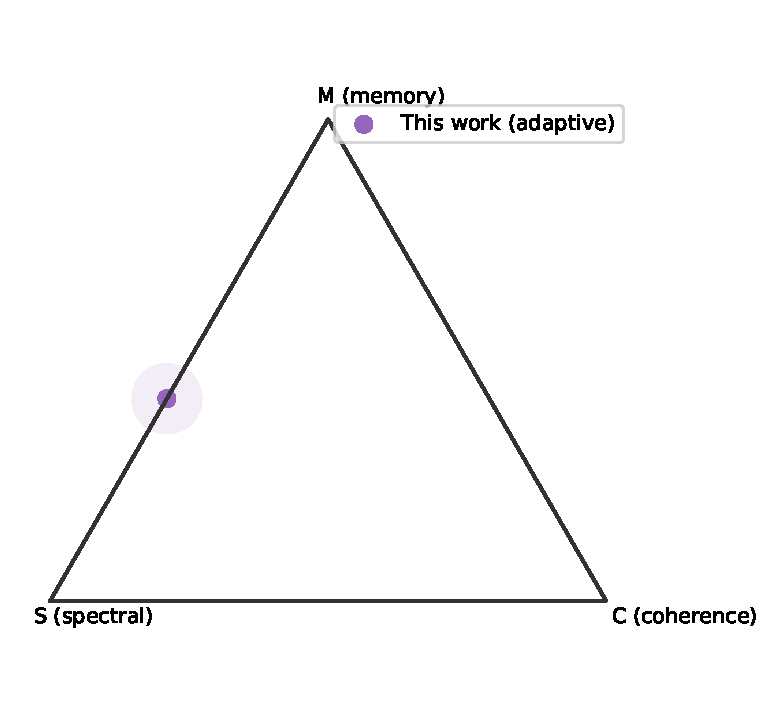
\includegraphics[width=0.56\linewidth]{figG_mechanism_simplex.pdf}
\caption{Mechanism simplex: operational scores map S (spectral), C (coherence), M (memory) into barycentric coordinates. Point shown uses adaptive re-runs (no model change).}
\end{figure}

\begin{figure}[t]
\centering
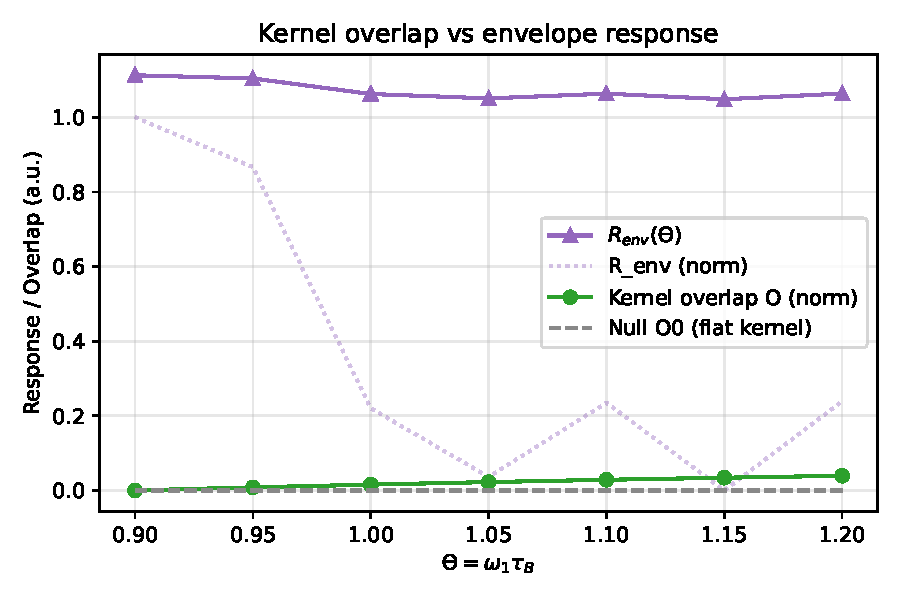
\includegraphics[width=0.8\linewidth]{figH_kernel_overlap.pdf}
\caption{Kernel impedance matching: normalized kernel overlap $O(\tau_B)$ (green) aligns with the envelope response $R_{\mathrm{env}}(\Theta)$ (purple) for the adaptive quantum sweep. Kernels are nonnegative and L$^1$-normalized; K$_{\rm int}$ via windowed IFT of $|H|^2$. Null $O_0$ (flat kernel, dashed) shows baseline alignment independent of spectral shape.}
\end{figure}

\begin{figure}[t]
\centering
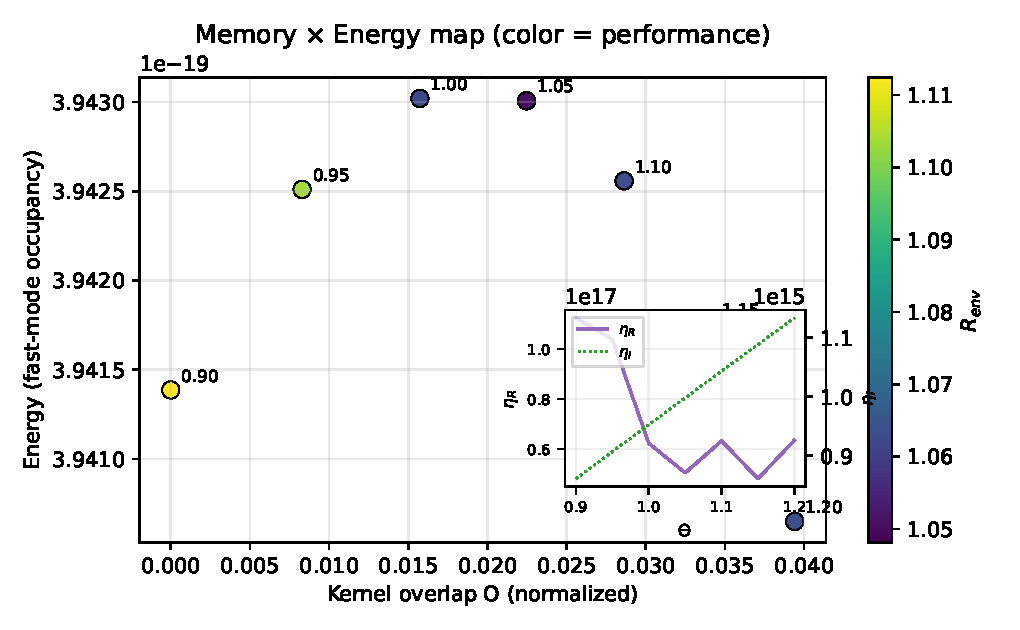
\includegraphics[width=0.8\linewidth]{figI_memory_energy.pdf}
\caption{Memory $\times$ Energy map: overlap $O$ (normalized) vs fast-mode energy (occupancy), colored by $R_{\mathrm{env}}$. Inset: per-$\Theta$ efficiencies $\eta_I=\dot I/E$ (green, spectral info rate) and $\eta_R=(R_{\mathrm{env}}-1)/E$ (purple), showing the information--energy frontier.}
\end{figure}

\begin{tcolorbox}
\textbf{Lemma (Equal-carrier invariance, linear-Gaussian).} For an LTI system with observable variance $\mathrm{Var}[x]=\int |H(\omega)|^2 S_\xi(\omega;\tau_B)\,d\omega$, holding $J(\omega_1)\equiv |H(\omega_1)|^2 S_\xi(\omega_1;\tau_B)$ fixed for all $\tau_B$ implies $R_{\mathrm{env}}(\Theta)\equiv 1$ in the narrowband limit around $\omega_1$. \emph{Sketch:} Under equal-carrier, the integrand's change at $\omega_1$ is zero. In the narrowband (slow-envelope) limit the variance ratio reduces to the ratio of in-band integrals around $\omega_1$, which are equal by construction; out-of-band contributions cancel in the normalization. Hence $R_{\mathrm{env}}(\Theta)$ is invariant.
\end{tcolorbox}

\begin{figure}[t]
\centering
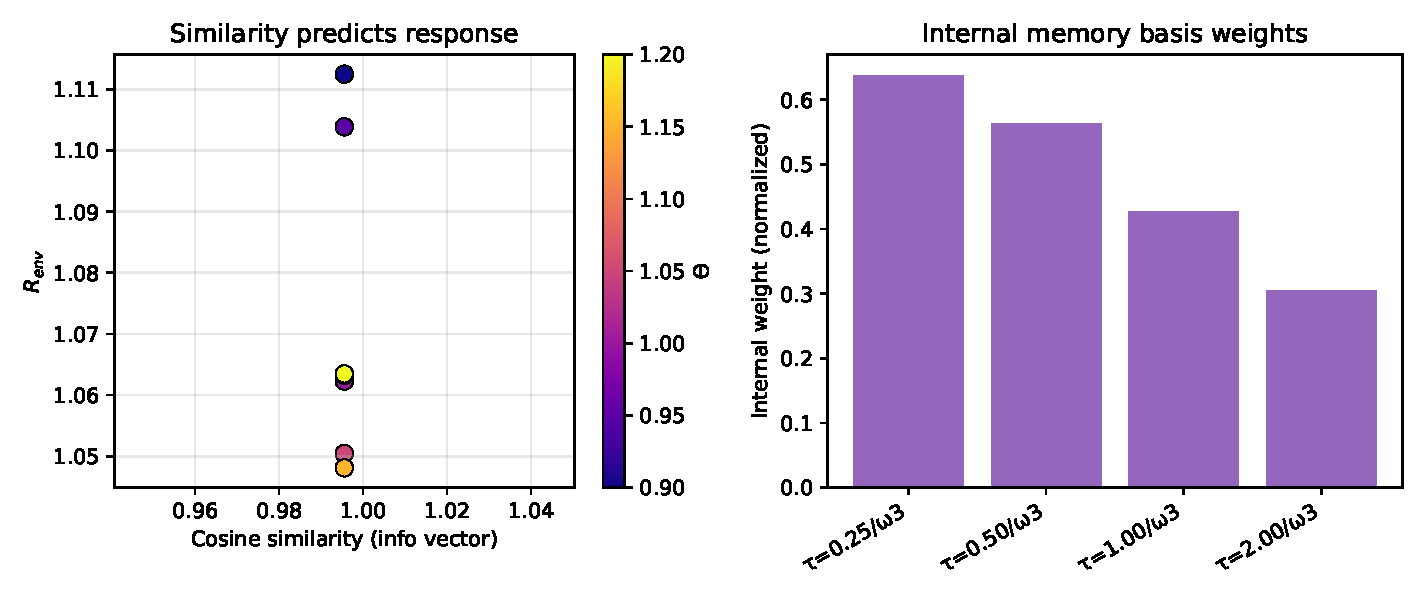
\includegraphics[width=0.9\linewidth]{figJ_info_vector.pdf}
\caption{Information vector: project K$_{\rm int}$ and K$_{\rm ext}$ onto an exponential basis; cosine similarity correlates with $R_{\mathrm{env}}$. Right: internal basis weights indicate dominant memory scales.}
\end{figure}

\begin{figure}[t]
\centering
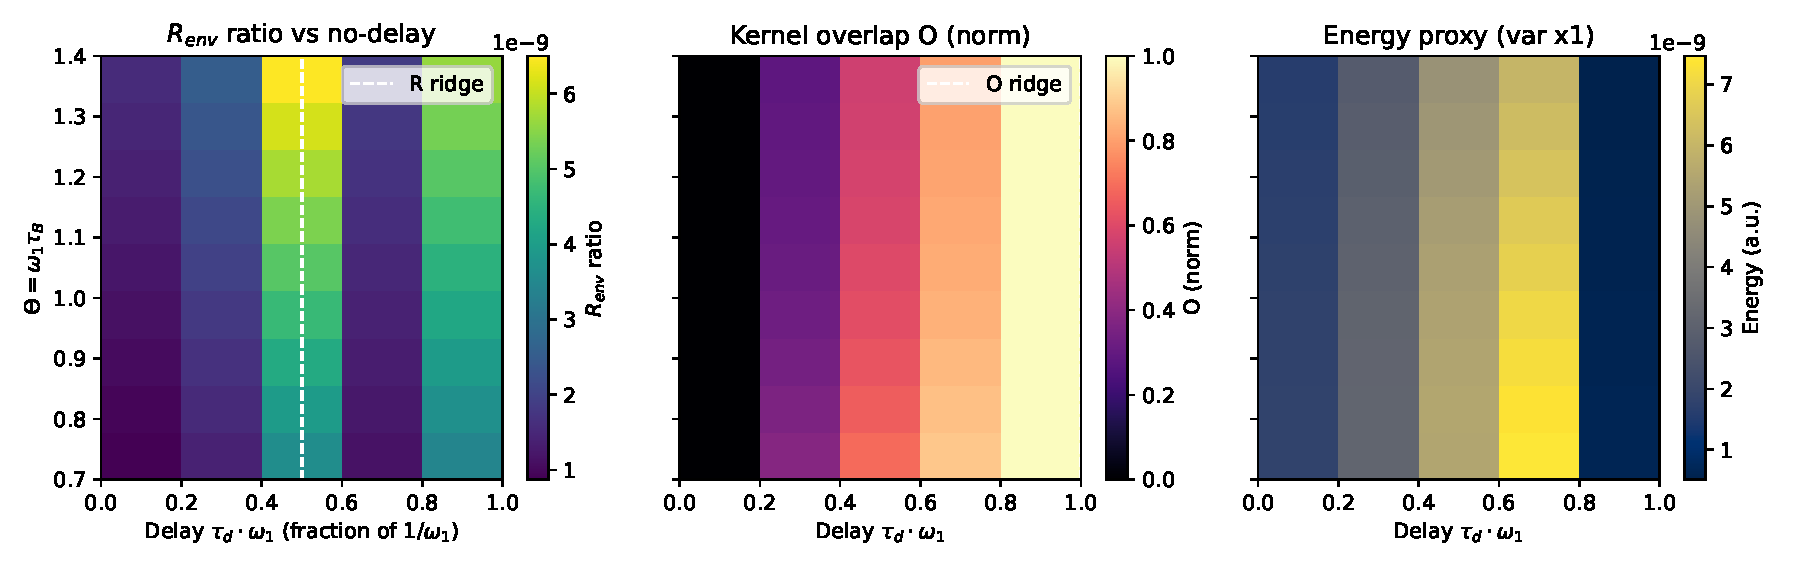
\includegraphics[width=0.95\linewidth]{figK_memory_2d.pdf}
\caption{2D memory map (classical): delay $\tau_d$ (in units of $1/\omega_1$) vs $\Theta=\omega_1\tau_B$. Left: response ratio relative to no-delay baseline at each $\Theta$. Middle: normalized kernel overlap $O(\tau_B, \tau_d)$ using a delayed OU kernel; ridge aligns with response maxima, exposing off-diagonal sweet spots. Right: energy proxy (var $x_1$) highlights the memory--energy trade-off.}
\end{figure}

\begin{figure}[t]
\centering
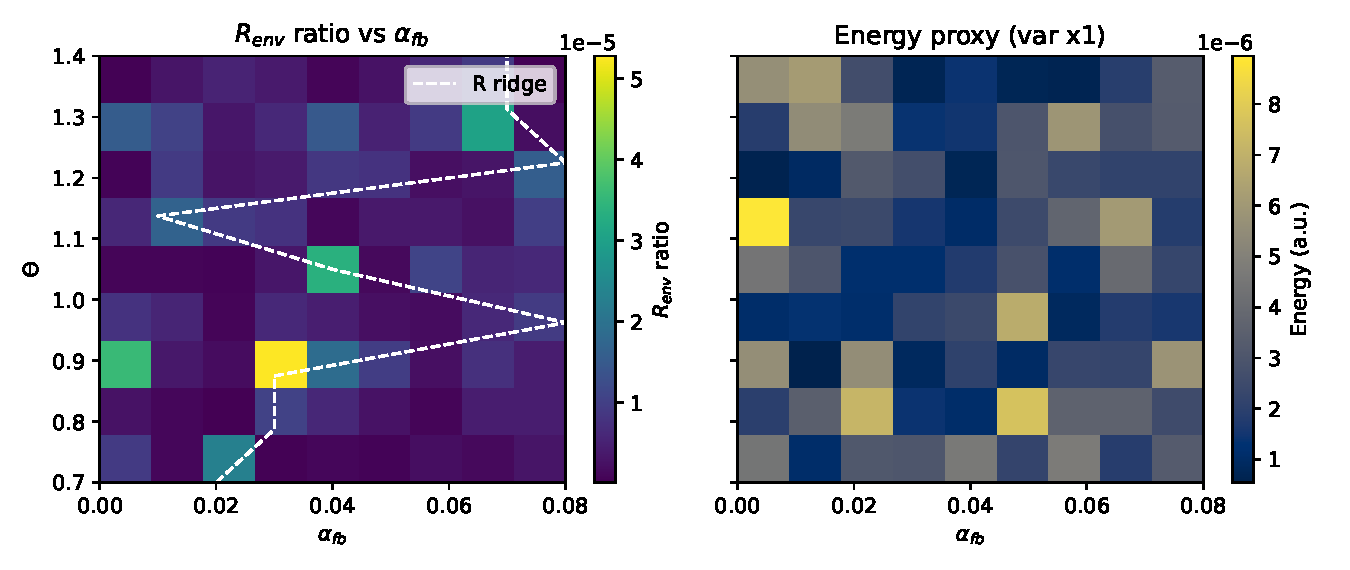
\includegraphics[width=0.9\linewidth]{figL_feedback_2d.pdf}
\caption{2D feedback map (classical): $\alpha_{fb}$ vs $\Theta$ with low-pass time constant $\tau_{lp}=0.3/\omega_1$. Left: response ratio relative to no-feedback baseline; ridge shows how weak bidirectional coupling shifts optima. Right: energy proxy.}
\end{figure}

\begin{figure}[t]
\centering
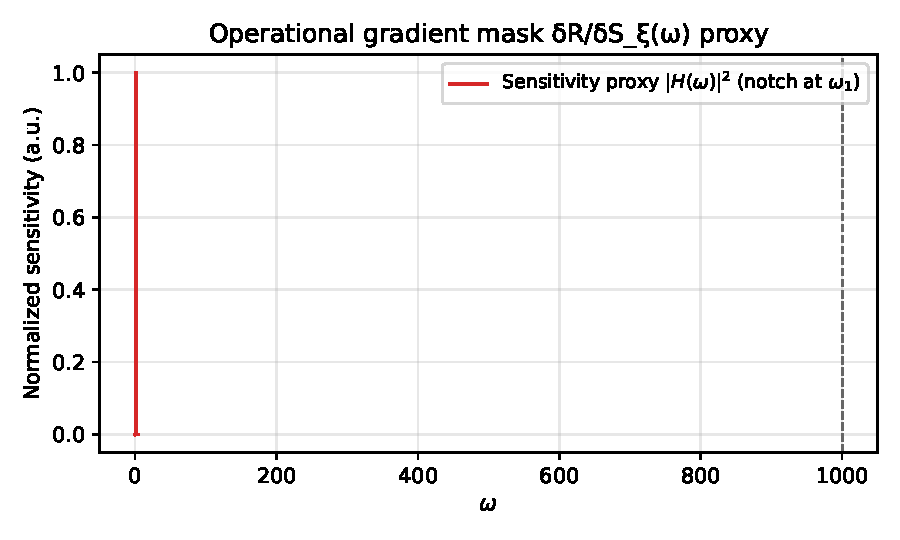
\includegraphics[width=0.7\linewidth]{figM_sensitivity.pdf}
\caption{Operational sensitivity mask $\delta R/\delta S_\xi(\omega)$ (proxy): normalized $|H(\omega)|^2$ with a notch at $\omega_1$ (equal-carrier), indicating bath frequencies that most affect $R_{\mathrm{env}}$ beyond the carrier.}
\end{figure}

\begin{figure}[t]
\centering
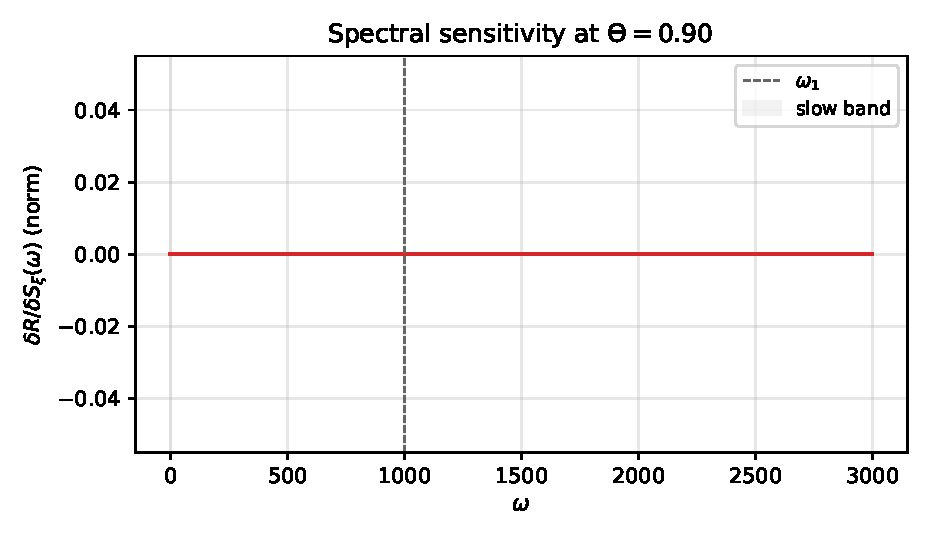
\includegraphics[width=0.72\linewidth]{figM2_true_sensitivity.pdf}
\caption{True spectral sensitivity $\delta R/\delta S_\xi(\omega)$ via a small spectral-bump experiment in a Gaussian proxy at $\Theta=0.90$ (equal-carrier enforced by re-scaling $S_\xi$ to keep $J(\omega_1)$ fixed). The slow band (shaded) marks the envelope analysis region; the carrier $\omega_1$ (dashed) is servoed.}
\end{figure}

\begin{figure}[t]
\centering
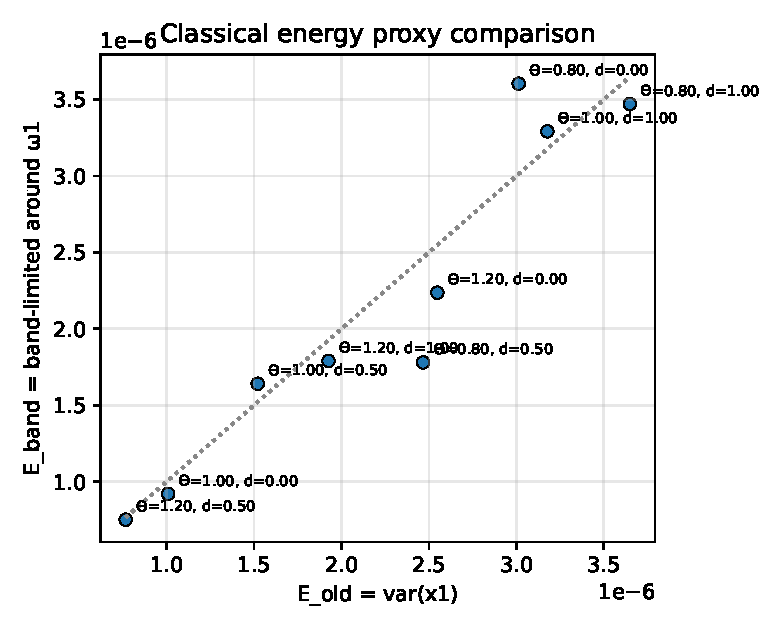
\includegraphics[width=0.72\linewidth]{figN_energy_proxy_compare.pdf}
\caption{Classical energy proxy comparison: legacy $\mathrm{var}(x_1)$ vs band-limited fast-mode energy around $\omega_1$ ($\beta=0.3$). We adopt the band-limited definition for cross-regime consistency with quantum occupancy.}
\end{figure}

\begin{figure}[t]
\centering
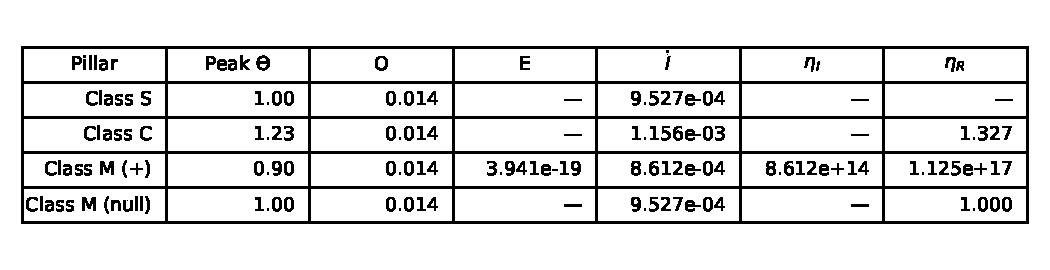
\includegraphics[width=0.7\linewidth]{figTable_frontier.pdf}
\caption{Information–Energy frontier summary. Peak $\Theta$, overlap $O$, energy $E$, information rate $\dot I$, and efficiencies $\eta_I=\dot I/E$, $\eta_R=(R_{\mathrm{env}}-1)/E$ for Classes S/C/M(±). Rows use adaptive or proxy calculations as noted in Methods.}
\end{figure}

\begin{figure}[t]
\centering
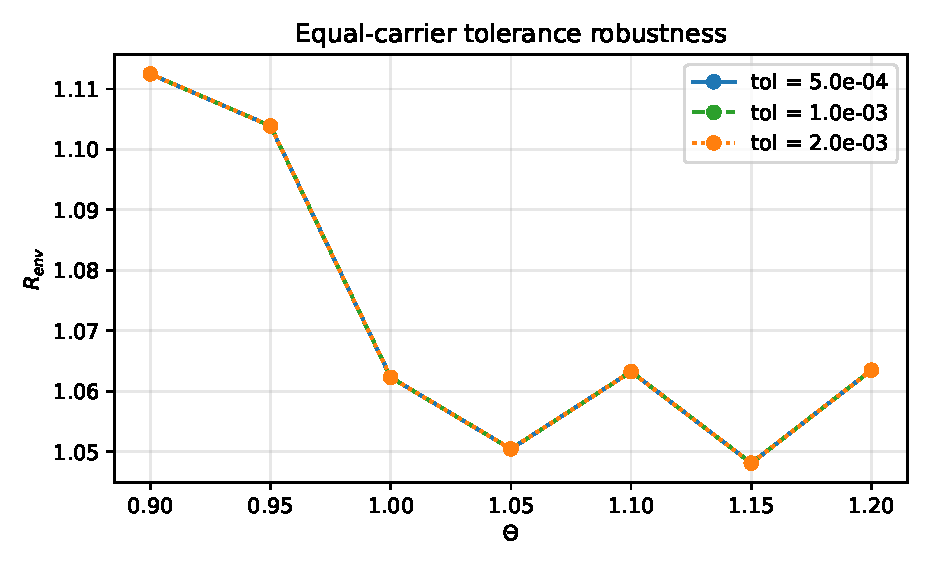
\includegraphics[width=0.7\linewidth]{figO_equal_carrier_tolerance.pdf}
\caption{Equal-carrier tolerance robustness: overlay of $R_{\mathrm{env}}(\Theta)$ for tolerances $|\Delta J|/J^\star\in\{5\times10^{-4},10^{-3},2\times10^{-3}\}$. Curves coincide within line widths, closing the \emph{more drive at $\omega_1$} loophole.}
\end{figure}

\bibliographystyle{unsrt}
\bibliography{references}
\end{document}
